%%%%%%%%%%%%%%%%%%%%%%%%%%%%%%%%%%%%%%%%%%%%%%%%%%%%%%%%%%%%%%%%%%%%%%%%%%
%% European Journal of Operational Research --- resubmission version
%% Built from main_trsc.tex (TS-2026-0253 desk-rejected; body is current
%% as of v2.4.6, includes Proposition 14 partition-pair certificate and
%% scale-up findings). Original main.tex retained unchanged for history.
%%%%%%%%%%%%%%%%%%%%%%%%%%%%%%%%%%%%%%%%%%%%%%%%%%%%%%%%%%%%%%%%%%%%%%%%%%

\documentclass[11pt]{article}
\usepackage[margin=1in]{geometry}
\usepackage{amsmath,amssymb,amsthm}
\usepackage{mathtools}
\usepackage{graphicx}
\usepackage{booktabs}
\usepackage{multirow}
\usepackage{natbib}
\usepackage{hyperref}
\usepackage{enumitem}
\usepackage{xcolor}
\usepackage[affil-it]{authblk}
\usepackage{setspace}
\usepackage{caption}
\usepackage{xr}
\externaldocument{supplementary_ejor}
\onehalfspacing

\captionsetup[table]{skip=8pt}
\hypersetup{colorlinks=true, linkcolor=blue!50!black, citecolor=blue!50!black, urlcolor=blue!60!black}
\emergencystretch=3em

\graphicspath{{../figures/}{../code/figures/}}

\theoremstyle{plain}
\newtheorem{theorem}{Theorem}
\newtheorem{lemma}[theorem]{Lemma}
\newtheorem{corollary}[theorem]{Corollary}
\newtheorem{proposition}[theorem]{Proposition}

\theoremstyle{definition}
\newtheorem{definition}[theorem]{Definition}
\newtheorem{example}[theorem]{Example}
\newtheorem{assumption}[theorem]{Assumption}

\theoremstyle{remark}
\newtheorem{remark}[theorem]{Remark}
\newtheorem{observation}[theorem]{Observation}

%% Custom math macros (verbatim from main_trsc.tex)
\newcommand{\F}{\mathcal{F}}
\newcommand{\Fp}{\mathcal{F}^{\mathrm{p}}}
\newcommand{\N}{N}
\newcommand{\CW}{\mathrm{CW}}
\newcommand{\cstar}{c^{\ast}}

\title{\textbf{Online Traveling Salesman Games: \\ Core Fragility and the Temporal Nucleolus under Dynamic Arrivals}}

\author[1]{Seyun Jeong\thanks{\texttt{jeongsseyyun@kitech.re.kr}}}
\author[1]{Hyunchul Tae\thanks{Corresponding author. \texttt{sage@kitech.re.kr}}}
\affil[1]{Korea Institute of Industrial Technology (KITECH), 303 Jeonghyu-ro, Dongnam-gu, Cheonan 31056, Republic of Korea}

\date{May 7, 2026}

\begin{document}
\maketitle

\begin{abstract}
\noindent Urban last-mile logistics---same-day delivery, ride-hailing, crowdsourced pickup---requires that the cost of a single shared tour be divided among customers whose identities are revealed only as the vehicle dispatches. Static cooperative routing models silently assume every customer is available from the outset, distorting fairness when arrivals are spread in time. We introduce the Online Traveling Salesman Game (Online TSG), in which the family of feasible coalitions is endogenously induced by the realized arrival-service process; the classical static game is recovered at simultaneous arrivals. We establish a general partition-pair sufficient condition for Core emptiness on the restricted family, with three a priori computable specializations (single-complement, balanced-complement, balanced-near-complement) ranged by sharpness. A bounded peak queue $k<n-1$ structurally blocks the three computable specializations; the general partition-pair mechanism via non-singleton splits remains active in this regime. Cooperative cost allocations are computed via a sequential cascade of linear programs (the Temporal Nucleolus). The single-complement threshold tightens at the Beardwood--Halton--Hammersley square-root rate as the number of customers grows. Synthetic experiments validate the framework on three fronts: the analytic thresholds are sharp on the realized empty Cores with no false positives; the structural blocking persists across dispatch policies; and the asymptotic tightening agrees with the predicted square-root rate at moderate sizes. Operationally, keeping the peak queue bounded suffices to preclude the dominant complement-coalition instability mechanisms.
\end{abstract}

\noindent\textbf{Keywords:} Routing; Cooperative games; Nucleolus; Core stability; Dynamic arrivals.

\section{Introduction}
\label{sec:introduction}

Urban last-mile logistics is characterized by requests that enter the system \emph{after} planning begins: online grocery orders, same-day parcels, ride-hail queues and crowdsourced pickups all share the feature that the identity of who will be served together with whom is not known until dispatch time \citep{pillac2013review,ausiello2001oltsp}. Operators nevertheless must share the routing cost among the customers who are eventually served on a joint tour, and the quality of this allocation shapes incentives for participation and pricing \citep{guajardo2016review}. Cooperative game theory, and specifically the Traveling Salesman Game (TSG) of \citet{potters1992tsg}, supplies the canonical framework in which a tour cost is divided so that no subset of customers has a strict incentive to defect; the Vehicle Routing Game (VRG) of \citet{gothe1996vrg,engevall2004heterogeneous} extends the idea to multi-vehicle settings. Classic applications of the VRG include school bus routing \citep{park2012schoolbus}, where the set of customers is fixed before the vehicle departs. Online counterparts arise naturally in same-day delivery and ride-hailing platforms, where requests arrive dynamically and the coalition of customers to be served jointly is revealed only during execution.

The classical TSG, however, is defined under the tacit assumption that every customer is available to be visited at any point of the tour: any coalition $S\subseteq N$ can be \emph{imagined} as a self-contained instance, and its characteristic cost $c(S)$ is the optimal traveling salesman problem (TSP) tour on $S\cup\{0\}$. In online settings, this counterfactual is not available: a coalition $S$ is operationally meaningful only if there exists a moment at which all members of $S$ have arrived but none have yet been served. Ignoring temporality hides a central source of instability. Two customers who arrive far apart in time are never candidates to be served together, and pretending that they form a coalition distorts fairness. Recent work on online cooperative games \citep{ge2024incentives,aziz2025participation,goyal2025temporal} has begun to address temporality but not in the routing context.

\paragraph{Research question.} What is the correct cooperative game-theoretic abstraction of the online traveling salesman problem, how does it compute, and---most importantly---when does it admit a stable allocation?

\paragraph{Why single vehicle.} The complement-coalition arguments of Corollary~\ref{cor:single-complement} and Corollaries~\ref{cor:balanced-complement} and~\ref{cor:balanced-near-complement} rely critically on the insertion identity $c(\{i\}) + c(N\setminus\{i\}) \geq \cstar(N)$---equivalently, splitting the grand tour into a singleton-and-complement pair cannot beat the joint TSP cost. In a metric symmetric single-vehicle setting this identity follows directly from the triangle inequality. In a multi-vehicle setting with capacity constraints, the identity can fail: when capacity binds, the optimal assignment of $S$ to multiple vehicles may yield strict cost savings over a single tour, and the characteristic function $c(S)$ becomes the sum of TSP tours under a fleet-assignment rule rather than a single tour cost. Under such cost structure, $c(\{i\}) + c(N\setminus\{i\})$ can lie either above or below $\cstar(N)$ depending on the capacity-binding regime, and the closed-form complement-pair thresholds developed here cease to be sufficient conditions for empty Core. We therefore scope the present paper to the single-vehicle Online TSG; the corresponding multi-vehicle Online VRG---combining the temporal feasibility family $\F$ with vehicle capacity and a fleet-assignment rule---is identified as future work (Section~\ref{sec:conclusion}).

\subsection{Contributions}

We make four contributions.
\begin{itemize}[leftmargin=1.5em]
\item[\textbf{C1.}] \emph{Model.} We define the Online TSG $(N, c, \F)$ by restricting coalitional stability constraints to the family $\F$ of proper sub-coalitions realizable under the realized arrival dynamics, with the grand coalition handled through the efficiency equality. This places the Online TSG within the taxonomy of restricted-cooperation games (Section~\ref{sec:related}) but with a novel source of restriction: $\F$ is not an exogenous graph or combinatorial structure but an endogenous random family induced by the arrival-service process. The classical static TSG is recovered as the special case where arrivals collapse to a single instant and the realized tour is optimal (Supplementary Proposition~\ref{prop:static-equiv}, Section~\ref{app:example-reduction}). Cooperative cost allocations on this restricted family are computed via a sequential linear program (LP) cascade (the Temporal Nucleolus, Section~\ref{sec:nucleolus}).
\item[\textbf{C2.}] \emph{Core theory under dynamics.} We provide one general partition-pair certificate (Theorem~\ref{thm:partition-pair} $r>r^{(P)}_{\min}$) for Temporal Core emptiness, with three a priori computable specializations: single-complement (Corollary~\ref{cor:single-complement} $r>r^{\ast\ast}$), balanced-complement on $B_{n-1}=\{N\setminus\{i\}\}$ (Corollary~\ref{cor:balanced-complement} $r>r^{\ast\ast\ast}$), and balanced-near-complement on the mixed collection $B_{n-1}\cup B_{n-2}$ (Corollary~\ref{cor:balanced-near-complement} $r>r^{(\diamond)}$). Corollary~\ref{cor:cor52} provides a structural obstruction for the three computable specializations; the general theorem additionally fires on non-singleton partition pairs at $k<n-1$ and certifies the 9 cases of Observation~\ref{obs:intermediate} that complement-only analyses leave open.
\item[\textbf{C3.}] \emph{Asymptotic refinement.} Under uniform coordinate sampling, $r^{\ast\ast}\to 1$ at rate $O(n^{-1/2})$ almost surely (Theorem~\ref{thm:asymptotic}); this explains the empirical smallness of $r^{\ast\ast}$ without reference to specific simulation parameters and ties the cooperative-game threshold to the classical Beardwood--Halton--Hammersley $\sqrt{n}$ scaling of the Euclidean TSP.
\item[\textbf{C4.}] \emph{Empirical calibration.} On 175 simulated instances across five coalition sizes and seven arrival patterns under three dispatch policies (525 policy-instance pairs), plus 45 scale-up instances up to $n=50$ and a 24-instance scale-invariance study (Supplementary Materials, Section~S2), we verify every theoretical claim. Under NN dispatch, Corollary~\ref{cor:single-complement} fires in 37 instances (all observed empty), Corollary~\ref{cor:balanced-complement} adds 11 balanced-complement certifications, and Corollary~\ref{cor:balanced-near-complement} adds 9 balanced-near-complement certifications (jointly 57 of 67 observed empties); the remaining 10 split as 1 near-complement residual (threshold-bound by $\approx 2\times 10^{-3}$) and 9 intermediate-coalition cases certified by Theorem~\ref{thm:partition-pair} (66 of 67 total). No false positives arise under any policy. The mean thresholds ($\bar r^{\ast\ast}=1.223$, $\bar r^{\ast\ast\ast}=1.096$) are sharper than the classical bound ($\bar r^{\ast}=4.351$) by factors of $3.56$ and $3.97$. Corollary~\ref{cor:cor52} holds analytically without exception: no instance with $k<n-1$ satisfies any of the three thresholds; the 9 intermediate-coalition empties all lie at $k<n-1$ under NN and vanish under cheapest-insertion and batch-reoptimization. The asymptotic decay $r^{\ast\ast}\to 1$ is consistent with Theorem~\ref{thm:asymptotic}'s $O(n^{-1/2})$ rate on the scale-up grid.
\end{itemize}

Operationally these results say: a bounded peak queue $k<n-1$---achievable via short service-time promises---eliminates all complement-coalition mechanisms (Corollary~\ref{cor:single-complement}, Corollaries~\ref{cor:balanced-complement} and~\ref{cor:balanced-near-complement}), covering the pathological ``morning batch'' regime. In the shallow-queue regime the intermediate-coalition mechanism of Observation~\ref{obs:intermediate} remains active but is policy-sensitive: observed only under nearest-neighbor dispatch and absent under cheapest-insertion or batch re-optimization (Section~\ref{ssec:policy}). Short service windows combined with moderately informed dispatch substantially improve empirical Core stability, though intermediate-coalition emptiness remains logically possible at high competitive ratios.

\paragraph{Structure.} The Online TSG is a single-vehicle cooperative game; this scope isolates the temporal coalition-feasibility structure of $\F$ from fleet-assignment confounds and is discussed further in Section~\ref{sec:conclusion} (where a multi-vehicle Online VRG is identified as future work). Section~\ref{sec:related} situates our work within the literature on static TSG/VRG, dynamic and rolling-horizon games, online cooperative games, and nucleolus computation. Section~\ref{sec:problem} formalizes the Online TSG. Section~\ref{sec:nucleolus} defines and computes the Temporal Nucleolus. Section~\ref{sec:theory} develops the Core theory. Section~\ref{sec:experiments} reports computational experiments, and Section~\ref{sec:conclusion} concludes.

\section{Literature review}
\label{sec:related}

We organize prior work along three streams and state, for each, the precise point of departure of our contribution.

\subsection{Cooperative Routing Games: Static, Dynamic, and Rolling-Horizon}
The cooperative TSP was initiated by \citet{potters1992tsg} with a characteristic function equal to the optimal TSP tour cost on the chosen coalition. \citet{tamir1989core} showed that the Core may be empty even on the Euclidean line, and the gap between fair and feasible allocations was quantified via approximation in \citet{faigle1998approximate} and \citet{blaser2008metric}. In parallel the Vehicle Routing Game (VRG) received a Nucleolus-based treatment by \citet{gothe1996vrg}, extended to heterogeneous fleets by \citet{engevall2004heterogeneous} and to time-window settings by \citet{tae2020vrgtw} and \citet{arroyo2024vrptw}. Most recently, \citet{lyu2025collaborative} study the collaborative berth allocation problem and compute stable cost allocations via row generation; their coalition family is static and determined by vessel identity rather than arrival dynamics, which is the source of restriction that differs from our setting. \citet{platz2015multidepot} extend the routing-plus-cooperative-game template to multi-depot Chinese postman problems, but with coalition family $2^N$ rather than a time-restricted $\F$. The Shapley value formulation of cooperative TSP under rolling horizons is treated by \citet{kimms2016rolling}, and a core-based variant by \citet{kimms2016core}; a broad survey is given by \citet{guajardo2016review}. \citet{ozener2008allocating} treat operational cost allocation among carriers in a collaborative transportation procurement network with a fixed carrier set. Closest in spirit to our work, \citet{ozener2013allocating} combine routing, cost allocation, and a temporal dimension in inventory routing; their temporality is a deterministic replenishment schedule rather than an online stochastic arrival process restricting $\F$. On the temporal side, \citet{kranich2005dynamic} proposed Core concepts for TU games played over discrete time, \citet{habis2010weak} defined the weak sequential Core to accommodate renegotiation, and \citet{lehrer2013dynamic} studied how the Core evolves as information unfolds. Our setting differs from these studies in a critical respect: every cited model either defines coalitions over the full customer set $2^N$ (so coalition identity is assumed known \emph{a priori}) or abstracts away the physical routing cost structure, describing coalitions combinatorially with exogenous values $v(S,t)$. We replace $2^N$ with the data-dependent family $\F$ of coalitions realizable under the online arrival process while retaining the metric TSP cost $c(S)$, so temporality enters through the \emph{admissibility} of coalitions and couples the game to the dispatch policy.

\subsection{Restricted Cooperation Games}

A parallel line of cooperative game theory, independent of the routing literature, studies games in which the set of formable coalitions is a \emph{strict subset} of $2^N$. \citet{myerson1977graphs} initiated this theme by treating coalitions as paths in an underlying communication graph, producing the graph-restricted game $(N, v^{c})$ in which $v^{c}(S)$ aggregates values of $S$'s connected components. \citet{faigle1989cores} generalized the framework to games on combinatorial structures (antimatroids, convex geometries, partitions), and \citet{bilbao2000} provided a unified treatment. \citet{algaba2001unified} connected Myerson's and Faigle's lines. More recent extensions handle permission structures \citep{gilles2010economic}, hierarchical coalition configurations, and the core of games on ordered structures \citep{grabisch2013core}. Computing the nucleolus of a restricted game is in general no harder than the unrestricted case and may be substantially easier, since the constraint count is $|\F|$ rather than $2^n-1$ \citep{schouten2019nucleolus}. Our work introduces a different source of restriction. In the restricted-cooperation literature above, feasibility is determined by an \emph{exogenous and time-invariant} structure---a graph, a partition, an antimatroid, or a permission relation---specified as part of the game's primitives. The Online TSG introduces a different source of restriction: feasibility is \emph{endogenously induced} by the realized dynamics of a stochastic arrival-service process. Formally, $\F$ is a data-dependent random family with $S\in\F$ iff customers in $S$ share a nonempty common waiting window $\CW(S)=\bigcap_{i\in S}[a_i,s_i]$ (Definition~\ref{def:feasible}). The resulting family $\F$ is closed under neither union nor intersection in general, and its shape depends on the arrival-order permutation, the queue-depth process, and the dispatch policy. Our theoretical contributions---the complement-coalition threshold $r^{\ast\ast}$ (Corollary~\ref{cor:single-complement}), the structural obstruction at bounded peak queue (Corollary~\ref{cor:cor52}), and the asymptotic tightening (Theorem~\ref{thm:asymptotic})---are specific to this time-induced restriction and have no direct counterpart in the graph-restricted or antimatroid literatures. We view the Online TSG as adding \emph{temporally-induced restricted cooperation} to the taxonomy of restricted-cooperation games.

A separate line of theoretical work relevant to our asymptotic analysis (Theorem~\ref{thm:asymptotic}) is the probabilistic theory of Euclidean combinatorial optimization, initiated by \citet{beardwood1959shortest} and systematized by \citet{steele1981subadditive,steele1997probability}. The Beardwood--Halton--Hammersley theorem characterizes the $\sqrt{n}$ scaling of the optimal Euclidean TSP tour, which in our setting controls the denominator of $r^{\ast\ast}$ and hence its asymptotic tightening. To the best of our knowledge, this asymptotic perspective on cooperative routing games is new: prior cooperative TSP and VRG studies \citep{potters1992tsg,gothe1996vrg,engevall2004heterogeneous,kimms2016core} treat the coalition cost as a fixed quantity rather than as a random variable with a known limit distribution.

\subsection{Online Cooperative Games and Nucleolus Computation}
\citet{bullinger2023online} studied online coalition formation under random arrival and dissolution. \citet{ge2024incentives} and \citet{zhang2025incentives} designed incentives for early arrival in online cost-sharing settings. \citet{aziz2025participation} characterized participation incentives for players entering over time. \citet{goyal2025temporal} introduce Temporal Cooperative Games, in which the characteristic function is indexed by time. Their worth $v(\pi)$ depends on the arrival sequence while coalitions remain unrestricted; our $c(S)$ is set-valued but coalitions are restricted to $\mathcal{F}$, an orthogonal axis of temporality. On the algorithmic side, \citet{schmeidler1969nucleolus} introduced the Nucleolus as the lexicographic minimizer of the excess vector; the sequential-LP approach that we adopt descends from Kohlberg's algorithm and its modernization by \citet{guajardo2015nucleolus}, with further scaling to large games by \citet{nguyen2016large}, Nucleolus-based ridesharing in \citet{lu2019ridesharing}, Nucleolus computation for the VRG with time windows (VRPTW) in \citet{tae2020vrgtw}, and a Core-targeted LP methodology for cooperative procurement in \citet{drechsel2010computing} that serves as an early precedent for the constraint-generation style we adapt to $\F$. \citet{vanzon2021joint} compute Core allocations for the Joint Network Vehicle Routing Game via a row-generation algorithm over a static coalition family; our sequential-LP cascade over the time-induced family $\F$ is methodologically analogous but applies to a different, dynamically restricted coalition structure. Our work differs from this online-game literature in two respects. First, \citet{bullinger2023online} formalize coalition \emph{formation} (which players group with whom) rather than cost sharing within a fixed grand coalition, so their stability concepts and ours address distinct strategic problems. Second, and common to the whole stream, none of these models equip the online coalition process with a TSP or routing cost structure; the inequalities that define our Temporal Core reflect exactly the geometric interactions among customers in the plane, allowing the sharp thresholds $r^{\ast\ast}$ and structural bound $k<n-1$ established in Section~\ref{sec:theory}. On the algorithmic side, our LP cascade is defined over $\F$ rather than $2^N\setminus\{\emptyset\}$: in sequential arrival regimes this can reduce the per-LP constraint count by more than an order of magnitude (Section~\ref{sec:experiments}).

\section{Problem Definition}
\label{sec:problem}

\subsection{Notation}
We consider a depot $0$ and $n$ customers $N = \{1,\ldots,n\}$, located in a metric space with symmetric travel cost $d$. A single vehicle leaves the depot, visits a subset of customers, and returns. Each customer $i\in N$ is associated with a random \emph{arrival time} $a_i \in \mathbb{R}_+$, revealed online, at which its request enters the system, and a \emph{service time} $s_i \ge a_i$ at which the vehicle first serves it in the realized execution. Table~\ref{tab:notation} collects the notation used throughout.

\begin{table}[t]
\centering
\caption{Notation.}
\label{tab:notation}
\small
\begin{tabular}{@{}lp{0.72\textwidth}@{}}
\toprule
Symbol & Meaning \\
\midrule
$N,\; n$ & Grand coalition of customers and its cardinality \\
$d(i,j)$ & Symmetric travel cost (metric) from $i$ to $j$ \\
$c(S)$ & Optimal TSP tour cost on $S\cup\{0\}$, \emph{time-independent} \\
$\cstar(N)$ & Grand-coalition TSP optimum (equals $c(N)$) \\
$a_i,\; s_i$ & Arrival and service time of customer $i$ \\
$U_t$ & Customers that have arrived by $t$ and are not yet served, $U_t=\{i:a_i\le t< s_i\}$ \\
$\F$ & Family of \emph{feasible coalitions}: $S\in\F$ iff $|S|=1$ or $\max_{i\in S} a_i < \min_{i\in S} s_i$ (Definition~\ref{def:feasible}) \\
$\CW(S)$ & Common window $\bigcap_{i\in S}[a_i, s_i]$ \\
$C(N)_{\text{online}}$ & Cost of the online tour realized by the dispatch policy \\
$r$ & Competitive ratio $C(N)_{\text{online}}/\cstar(N)$ \\
$\delta_i$ & $c(\{i\})+c(N\setminus\{i\})-\cstar(N)$ \\
$r^{\ast\ast}$ & $1+\min_{i:\,N\setminus\{i\}\in\F}\delta_i/\cstar(N)$: tight threshold (Cor.~\ref{cor:single-complement}); undefined if no such $i$ exists; computable a priori from coordinates \\
$r^{\ast\ast\ast}$ & $\bigl(\sum_{i\in N} c(N\setminus\{i\})\bigr)/\bigl((n-1)\,\cstar(N)\bigr)$: balanced-complement threshold (Cor.~\ref{cor:balanced-complement}); requires $B_{n-1}\subseteq\F$; computable a priori from coordinates \\
$r^{(\diamond)}_{\min}$ & LP optimum of Bondareva--Shapley over $B_{n-1}\cup B_{n-2}$ (Cor.~\ref{cor:balanced-near-complement}); requires $B_{n-1}\cup B_{n-2}\subseteq\F$; post-hoc LP solve required \\
$r^{(P)}_{\min}$ & Partition-pair threshold $\min_{(S,N\setminus S)\in\F^{2}}\,(c(S)+c(N\setminus S))/\cstar(N)$ (Thm.~\ref{thm:partition-pair}); post-hoc, via partition enumeration or Core-LP dual \\
$r^{\ast}$ & $\sum_i c(\{i\})/\cstar(N)$: Remark~\ref{rem:rstar} upper bound \\
$k$ & $\max_t |U_t|$: peak size of the waiting queue \\
\bottomrule
\end{tabular}
\end{table}

\subsection{Feasible coalitions and the characteristic function}

The starting point is that the characteristic cost $c(S)$ of a coalition is \emph{defined in the same way as in the static TSG}: it is the cost of the optimal TSP tour on $S\cup\{0\}$ irrespective of time. Temporality enters only through the admissibility of coalitions.

\begin{definition}[Common waiting window]
\label{def:cw}
For a coalition $S\subseteq N$,
$\CW(S) := \bigcap_{i\in S} [a_i, s_i]$.
\end{definition}

\begin{definition}[Feasible coalition]
\label{def:feasible}
A nonempty coalition $S\subseteq N$ is \emph{feasible} under the realized arrival/service sequence $(a, s)$ if either $|S|=1$, or $|S|\ge 2$ and $\max_{i\in S} a_i < \min_{i\in S} s_i$. Let
\[
\F \;:=\; \bigl\{S\subseteq N : S\neq\emptyset,\ \text{$|S|=1$ or } \max_{i\in S} a_i < \min_{i\in S} s_i\bigr\}
\]
denote the family of feasible coalitions. Equivalently, $S\in\F$ iff $\CW(S)$ is nonempty \emph{and} has nonempty interior whenever $|S|\ge 2$, i.e.\ iff there exists $t$ with $a_i\le t<s_i$ for every $i\in S$ or $S$ is a singleton.
\end{definition}

Under the closed-interval convention of Definition~\ref{def:cw}, $\CW(\{i\})=[a_i,s_i]\ni a_i$ is automatically nonempty for every $i\in N$, even when the vehicle reaches $i$ at its arrival instant (i.e.\ $s_i=a_i$), so singletons are always feasible without an auxiliary convention. For $|S|\ge 2$, the strict inequality $\max_{i\in S}a_i<\min_{i\in S}s_i$ used in Supplementary Lemma~\ref{lem:lemma51} and in our implementation identifies the open interior of $\CW(S)$ within which every member strictly co-waits before any service begins; boundary configurations with $\max a_i=\min s_i$ have Lebesgue measure zero under continuous arrival distributions and correspond to a member arriving at the instant another member's service begins, and are excluded on operational grounds. The grand coalition $N\in\F$ whenever all $n$ customers are queued simultaneously. We write $\Fp := \F\setminus\{N\}$ for the family of \emph{proper} feasible coalitions; the Temporal Core and Temporal Nucleolus are defined on $\Fp$, with $N$ entering only through the efficiency equality \citep{myerson1977graphs,bilbao2000}.

The family $\F$ is determined ex post by the realized arrival-service sequence $(a,s)$, where $s$ is the realized service time under the deployed dispatch policy. The Online TSG Core is therefore an ex-post, policy-induced stability concept rather than a counterfactual one. The sensitivity of $\F$ to the choice of dispatch policy is taken up further in Section~\ref{sec:conclusion}.

\begin{definition}[Online TSG]
\label{def:online-tsg}
An \emph{Online Traveling Salesman Game} is a triple $(N, c, \F)$ where $N$ is the customer set, $c:2^N\setminus\{\emptyset\}\to\mathbb{R}_+$ is the TSP characteristic cost defined on every nonempty subset, with core stability constraints imposed only for $S\in\Fp$, and $\F\subseteq 2^N\setminus\{\emptyset\}$ is the family from Definition~\ref{def:feasible}.
\end{definition}

An \emph{allocation} is a vector $x\in\mathbb{R}^n$ with $\sum_i x_i = C(N)_{\text{online}}$, where $C(N)_{\text{online}}$ denotes the realized online tour cost. The \emph{Temporal Core} is
\[
\begin{aligned}
\mathrm{Core}(N,c,\F) := {} & \bigl\{ x\in\mathbb{R}^n : \\
& \quad \textstyle\sum_i x_i = C(N)_{\text{online}}, \\
& \quad \textstyle\sum_{i\in S} x_i \le c(S)\ \forall S\in\Fp \bigr\}.
\end{aligned}
\]
When $C(N)_{\text{online}} = \cstar(N)$, this definition coincides with the classical \citet{potters1992tsg} static TSG Core on the same constraint family. In general, the online overhead $C(N)_{\text{online}}-\cstar(N)\ge 0$ raises the efficiency budget above the minimum grand-coalition cost; Table~\ref{tab:static-vs-temporal} summarizes the contrast, and the competitive ratio $r$ (defined below) quantifies this overhead.

\paragraph{Characteristic cost versus realized cost.} The characteristic function $c(S)$ is the time-independent optimal TSP tour on $S\cup\{0\}$, matching the classical \citet{potters1992tsg} definition. The realized online tour cost $C(N)_{\text{online}}$, by contrast, is the total travel distance of the tour actually executed by the online dispatch policy, which may exceed $\cstar(N)$ because the online policy cannot anticipate future arrivals; in general $C(N)_{\text{online}} \ge \cstar(N)$. We use $\sum_i x_i = C(N)_{\text{online}}$ as the efficiency budget because this is the cost the platform must actually allocate; the competitive ratio $r = C(N)_{\text{online}}/\cstar(N)$ measures this overhead. The cost terms entering $r^{\ast\ast}$ (Corollary~\ref{cor:single-complement}) are geometric through $c(\{i\})$, $c(N\setminus\{i\})$, and $\cstar(N)$, while applicability and the feasible-complement index set $\{i:\,N\setminus\{i\}\in\F\}$ are determined by the realized arrival-service windows.

\begin{table}[t]
\centering
\caption{Static TSG versus Online TSG.}
\label{tab:static-vs-temporal}
\small
\begin{tabular}{@{}lll@{}}
\toprule
 & Static TSG \citep{potters1992tsg} & Online TSG (this paper) \\
\midrule
Coalitions considered & All $S\subseteq N$, $S\neq\emptyset$ & $S\in\F$ \\
Characteristic function & $c(S)$ = TSP on $S\cup\{0\}$ & Same \\
Core constraints & $2^n-1$ & $|\F|\le 2^n-1$ \\
Recovers classical TSG & --- & Yes, when $\F=2^N\setminus\{\emptyset\}$ \\
\bottomrule
\end{tabular}
\end{table}

\paragraph{Illustrative example.} Supplementary Section~\ref{app:example-reduction} works through the Online TSG on the first five customers of the Solomon C101 benchmark \citep{solomon1987benchmarks}: the realized service timeline is fully sequential ($k=1$), all five singletons are feasible while no complement coalition is, and the Temporal Nucleolus reduces to an equal-excess allocation across the singleton constraints, illustrating how temporal restriction discards 26 of the 31 static-TSG inequalities while preserving Core existence.

\section{Cost Allocation: The Temporal Nucleolus}
\label{sec:nucleolus}

Even when the Core is nonempty it is typically a polytope, and one needs a selection rule. We adopt the nucleolus of \citet{schmeidler1969nucleolus}, adapted to the feasible family $\F$.

\subsection{Definition}
For an allocation $x$ and $S\in\Fp$, the \emph{excess} is $e(S, x) := \sum_{i\in S} x_i - c(S)$. Let $\theta(x)$ be the vector $(e(S,x))_{S\in\Fp}$ sorted in non-increasing order.

\begin{definition}[Temporal Nucleolus]
\label{def:tnu}
The Temporal Nucleolus of $(N, c, \F)$ is
\[
\begin{aligned}
\mathrm{TNu}(N,c,\F) := \arg\!\min{}^{\text{lex}} \bigl\{ \theta(x) : {} & \textstyle\sum_i x_i \\
& = C(N)_{\text{online}}\bigr\},
\end{aligned}
\]
where the minimization is lexicographic over the sorted excess vector.
\end{definition}

\subsection{Sequential LP computation}

Following the standard technique of \citet{guajardo2015nucleolus}, the Temporal Nucleolus is computed by solving at most $|\Fp|$ linear programs. At stage $q$ the LP
\begin{equation}
\label{eq:lp-q}
\begin{aligned}
\min_{x,\varepsilon} \;& \varepsilon \\
\text{s.t. } \;& \sum_{i} x_i = C(N)_{\text{online}}, \\
& \sum_{i\in S} x_i - c(S) \le \varepsilon \qquad \forall S\in\Fp\setminus\Fp_{<q}, \\
& \sum_{i\in S} x_i - c(S) = \varepsilon_{q(S)}^{\ast} \qquad \forall S\in\Fp_{<q},
\end{aligned}
\end{equation}
determines the $q$-th largest coordinate of $\theta$. Here $\Fp_{<q}$ collects the coalitions whose excess was fixed at earlier stages with optimal value $\varepsilon_{q(S)}^{\ast}$. Finiteness of $\Fp$ guarantees termination in at most $|\Fp|$ stages; each LP has $n+1$ variables and $|\Fp|+1$ constraints.

\paragraph{Algorithmic scope.} All Core-stability results of this paper depend only on the first-stage LP $\varepsilon_1^{\ast}$; tie-breaking and primal-degeneracy refinements are needed only for the full Nucleolus point and are described in Supplementary Section~\ref{app:algorithmic-details}.

The restriction from $2^N\setminus\{\emptyset\}$ to $\F$ materially reduces problem size whenever arrivals are spread in time. Section~\ref{sec:experiments} reports empirically $|\F|/(2^n-1)$ as low as $0.061$ for heavily sequential patterns.

\subsection{Reduction to the static game at simultaneous arrivals}

When all customers arrive simultaneously and the realized tour is additionally optimal ($C(N)_{\text{online}}=\cstar(N)$), the Temporal Nucleolus reduces to the classical static Nucleolus of \citet{potters1992tsg} on the unrestricted coalition family $2^N\setminus\{\emptyset\}$ (Supplementary Proposition~\ref{prop:static-equiv}, Section~\ref{app:example-reduction}). Numerical verification on 25 pattern-A instances of the main grid confirms coordinate-wise coincidence to within $10^{-9}$. The Online TSG is therefore a proper generalization, with the static theory recovered as the $k=n$ extremal case where the peak waiting queue contains every customer at once.

\section{Theoretical Results}
\label{sec:theory}

We now develop the Core theory. Section~\ref{ssec:empty} establishes conditions under which the Temporal Core is \emph{empty}; Section~\ref{ssec:survive} gives conditions under which it is guaranteed \emph{nonempty}. Section~\ref{ssec:discussion} discusses the relationships between the parameters $r$, $r^{\ast\ast}$, $k$, and the queue dynamics.

\subsection{Conditions under which the Core vanishes}
\label{ssec:empty}

\paragraph{Hierarchy and computability.} The general result is Theorem~\ref{thm:partition-pair} (partition-pair certificate, used \emph{post-hoc} via partition enumeration or Core-LP dual). Three specializations admit \emph{a priori} computable thresholds in ascending sharpness: single-complement (Corollary~\ref{cor:single-complement}, $r>r^{\ast\ast}$, coordinate-only), balanced-complement (Corollary~\ref{cor:balanced-complement}, $r>r^{\ast\ast\ast}$, coordinate-only), and balanced-near-complement (Corollary~\ref{cor:balanced-near-complement}, $r>r^{(\diamond)}_{\min}$, LP on $B_{n-1}\cup B_{n-2}$). Operationally, $r^{\ast\ast}$ and $r^{\ast\ast\ast}$ are the informative a priori thresholds; the general theorem additionally fires on non-singleton partition pairs at $k<n-1$ where the three specializations are structurally vacuous (Corollary~\ref{cor:cor52}; Observation~\ref{obs:intermediate}).

\begin{table}[h]
\centering
\caption{Hierarchy of sufficient conditions for an empty Temporal Core, in ascending sharpness. Statements and proofs follow in Theorem~\ref{thm:partition-pair} (general) and its specializations Corollaries~\ref{cor:single-complement},~\ref{cor:balanced-complement},~\ref{cor:balanced-near-complement}; the asymptotic refinement is Theorem~\ref{thm:asymptotic}.}
\label{tab:threshold-hierarchy}
\small
\begin{tabular}{@{}lllll@{}}
\toprule
Mechanism & Threshold & Hypothesis on $\F$ & Computability & Sharpness ($r^{\ast}/\cdot$, NN grid) \\
\midrule
Singleton (Rem.~\ref{rem:rstar}) & $r > r^{\ast}$ & none & a priori & $1$ (baseline) \\
Single-complement (Cor.~\ref{cor:single-complement}) & $r > r^{\ast\ast}$ & $\exists\, i:\, N\setminus\{i\}\in\F$ & a priori & $\sim 3.56$ \\
Balanced-complement (Cor.~\ref{cor:balanced-complement}) & $r > r^{\ast\ast\ast}$ & $B_{n-1}\subseteq\F$ & a priori & $\sim 3.97$ \\
Balanced-near-complement (Cor.~\ref{cor:balanced-near-complement}) & $r > r^{(\diamond)}_{\min}$ & $B_{n-1}\cup B_{n-2}\subseteq\F$ & post-hoc LP & --- \\
General partition-pair (Thm.~\ref{thm:partition-pair}) & $r > r^{(P)}_{\min}$ & $\exists\,(S,N\setminus S)\in\F^{2}$ & post-hoc LP/enum & --- \\
\bottomrule
\end{tabular}
\end{table}

\begin{remark}[Necessary super-additivity failure]
\label{rem:remark1}
\label{rem:rstar}
A trivial necessary condition for Temporal Core emptiness comes from super-additivity failure of the singleton constraints: if $C(N)_{\text{online}} > \sum_{i\in N} c(\{i\})$, equivalently $r > r^{\ast} := \sum_i c(\{i\})/\cstar(N)$, then no allocation can simultaneously satisfy the efficiency equality $\sum_i x_i = C(N)_{\text{online}}$ and the singleton constraints $x_i \le c(\{i\})$, so the Temporal Core is empty. This bound is rarely tight in practice ($r^{\ast}$ is typically in the range $3$--$4$ while the competitive ratio of reasonable online policies is close to $1$); we sharpen it substantially by exploiting complement coalitions $N\setminus\{i\}$. The feasibility characterization of complement coalitions and a structural consequence under fully sequential arrivals are recorded as Supplementary Lemmas~\ref{lem:lemma51} and~\ref{lem:lemma52} (Section~\ref{app:complement-feasibility-lemmas}); we cite them where used.
\end{remark}

%% Numbering counter advanced by 3 to preserve historical numbering of
%% the original Theorem 9 / now Corollary 9 (single-complement); Proposition 14
%% / now Theorem 14 (general partition-pair) automatically inherits position 14.
\addtocounter{theorem}{3}
\begin{corollary}[Single-complement specialization]
\label{cor:single-complement}
Assume that $N\setminus\{i\}\in\F$ for some $i\in N$. Let
\[
\begin{aligned}
\delta_i & := c(\{i\}) + c(N\setminus\{i\}) - \cstar(N), \\
r^{\ast\ast} & := 1 + \min_{i:\,N\setminus\{i\}\in\F} \delta_i/\cstar(N).
\end{aligned}
\]
If $r = C(N)_{\text{online}}/\cstar(N) > r^{\ast\ast}$, then the Temporal Core is empty.
\end{corollary}

\begin{proof}
Let $i^{\star}\in\arg\min_{i:\,N\setminus\{i\}\in\F} \delta_i$. Both $\{i^{\star}\}\in\F$ (singletons are always feasible) and $N\setminus\{i^{\star}\}\in\F$. Suppose, for contradiction, that $x$ lies in the Temporal Core. The two core inequalities read
\begin{align}
x_{i^{\star}} &\le c(\{i^{\star}\}), \label{eq:sing}\\
\sum_{j\neq i^{\star}} x_j &\le c(N\setminus\{i^{\star}\}).\label{eq:comp}
\end{align}
Adding~\eqref{eq:sing} and~\eqref{eq:comp} gives $\sum_{j\in N} x_j \le c(\{i^{\star}\}) + c(N\setminus\{i^{\star}\}) = \cstar(N) + \delta_{i^{\star}}$. But the efficiency constraint forces $\sum_j x_j = C(N)_{\text{online}} = r\cdot \cstar(N)$. Hence $r\le 1 + \delta_{i^{\star}}/\cstar(N) = r^{\ast\ast}$, contradicting the hypothesis $r>r^{\ast\ast}$.
\end{proof}

This is the $|S|=1$ specialization of Theorem~\ref{thm:partition-pair} below (Proposition~14 in the original numbering). Because $\min_i \delta_i$ is typically small ($\delta_i=0$ corresponds to $\{i\},N\setminus\{i\}$ partitioning the grand tour with no overhead), $r^{\ast\ast}$ is close to $1$ and thus an operationally informative threshold. We stress that Corollary~\ref{cor:single-complement} is tight only \emph{within the single-complement mechanism}: even when no single complement $N\setminus\{i\}$ alone violates the Core, a balanced collection of complements can; this is captured by Corollary~\ref{cor:balanced-complement} below. Intermediate-size coalitions $S$ with $|S|\in\{2,\ldots,n-2\}$ can also independently violate the Core inequality $\sum_{i\in S} x_i \le c(S)$; Section~\ref{sec:experiments} exhibits observed cases of both mechanisms (Remark~\ref{rem:near-complement} and Section~\ref{ssec:cor16}).

\begin{corollary}[Balanced-complement specialization]
\label{cor:balanced-complement}
Let $n\ge 2$ and suppose every complement coalition is feasible, i.e., $N\setminus\{i\}\in\F$ for all $i\in N$. Define
\[
r^{\ast\ast\ast} \;:=\; \frac{1}{n-1}\cdot\frac{\sum_{i\in N} c(N\setminus\{i\})}{\cstar(N)}.
\]
If $r = C(N)_{\text{online}}/\cstar(N) > r^{\ast\ast\ast}$, then the Temporal Core is empty.
\end{corollary}

\begin{proof}
Suppose $x\in\mathrm{Core}(N,c,\F)$. For each $i\in N$, the Core constraint on $N\setminus\{i\}$ reads $\sum_{j\ne i} x_j \le c(N\setminus\{i\})$. Summing over $i\in N$ and exchanging the order of summation gives
\[
(n-1)\sum_{j\in N} x_j \;=\; \sum_{i\in N}\sum_{j\ne i} x_j \;\le\; \sum_{i\in N} c(N\setminus\{i\}).
\]
The efficiency equality $\sum_j x_j = C(N)_{\text{online}}$ yields $(n-1)\,C(N)_{\text{online}} \le \sum_i c(N\setminus\{i\})$. Dividing by $(n-1)\,\cstar(N)$ produces $r \le r^{\ast\ast\ast}$, contradicting $r>r^{\ast\ast\ast}$.
\end{proof}

This is the balanced-collection specialization of Theorem~\ref{thm:partition-pair} averaged uniformly over the $n$ singleton-complement partition pairs (Proposition~10 in the original numbering). The collection $\{N\setminus\{i\}\}_{i\in N}$ is balanced with weights $\lambda_i = 1/(n-1)$ (each player appears in exactly $n-1$ complements), so Corollary~\ref{cor:balanced-complement} is the Bondareva--Shapley criterion \citep{shapley1971core} specialised to this collection. Corollary~\ref{cor:single-complement} and Corollary~\ref{cor:balanced-complement} are incomparable in general: Corollary~\ref{cor:single-complement} depends on the minimum $\delta_i$ and fires when a single complement is cheap, whereas Corollary~\ref{cor:balanced-complement} averages the complement costs and fires when the balanced collection as a whole is cheap. Section~\ref{sec:experiments} exhibits instances where $r > r^{\ast\ast\ast}$ but $r\le r^{\ast\ast}$, so the Core is certified empty by Corollary~\ref{cor:balanced-complement} alone.

\begin{corollary}[Fully sequential arrivals disarm Corollary~\ref{cor:single-complement}]
\label{cor:cor51}
If arrivals are fully sequential in the sense of Supplementary Lemma~\ref{lem:lemma52}, then Corollary~\ref{cor:single-complement} is vacuous: no $N\setminus\{i\}$ is feasible, so its hypothesis cannot hold.
\end{corollary}

\begin{proof}
Direct from Supplementary Lemma~\ref{lem:lemma52} and the hypothesis of Corollary~\ref{cor:single-complement}. The same argument rules out Corollary~\ref{cor:balanced-complement}'s hypothesis, which additionally requires every $N\setminus\{i\}$ to be feasible; the balanced-complement mechanism is likewise blocked under fully sequential arrivals.
\end{proof}

\begin{remark}[Near-complement mechanism]
\label{rem:near-complement}
Beyond Corollary~\ref{cor:single-complement} and Corollary~\ref{cor:balanced-complement}, we observe main-grid instances (10 of 175 under the NN policy) where the Temporal Core is empty, both thresholds are vacuous, and the binding constraints in the Core LP mix size-$(n-1)$ and size-$(n-2)$ coalitions simultaneously. Corollary~\ref{cor:balanced-near-complement} below formalises this mechanism as a Bondareva--Shapley sufficient condition on the mixed collection $B_{n-1}\cup B_{n-2}$; it fires on 9 of the 10 observed cases (Section~\ref{ssec:cor16}, Table~\ref{tab:thm5}; Supplementary Materials Section~S4).
\end{remark}

\begin{corollary}[Balanced-near-complement specialization]
\label{cor:balanced-near-complement}
Let $n\ge 3$, $B_{n-1}=\{N\setminus\{i\}:i\in N\}$, and $B_{n-2}=\{N\setminus\{i,j\}:i\neq j\in N\}$. Assume $\F\supseteq B_{n-1}\cup B_{n-2}$, i.e.\ every size-$(n-1)$ and size-$(n-2)$ coalition is feasible. Let $\lambda=(\lambda_S)_{S\in B_{n-1}\cup B_{n-2}}$ be a vector of non-negative weights satisfying the balancing condition
\[
\sum_{S\ni i}\lambda_S \;=\; 1 \qquad \text{for every } i\in N,
\]
where the sum is taken over all $S\in B_{n-1}\cup B_{n-2}$ containing $i$. Define
\[
r^{(\diamond)}(\lambda) \;:=\; \frac{\sum_{S\in B_{n-1}\cup B_{n-2}}\lambda_S\,c(S)}{\cstar(N)}.
\]
If the realized competitive ratio $r = C(N)_{\text{online}}/\cstar(N)$ satisfies $r>r^{(\diamond)}(\lambda)$ for some such $\lambda$, then $\mathrm{Core}(N,c,\F)=\emptyset$.
\end{corollary}

\begin{proof}
Suppose for contradiction that $x\in\mathrm{Core}(N,c,\F)$. The feasibility hypothesis $\F\supseteq B_{n-1}\cup B_{n-2}$ ensures that for every $S\in B_{n-1}\cup B_{n-2}$ the Temporal Core stability inequality
\begin{equation}
\label{eq:bnc-core}
\sum_{i\in S}x_i \;\le\; c(S)
\end{equation}
is imposed. Multiplying~\eqref{eq:bnc-core} by the non-negative weight $\lambda_S$ and summing over $S\in B_{n-1}\cup B_{n-2}$ yields
\[
\sum_{S\in B_{n-1}\cup B_{n-2}}\lambda_S \sum_{i\in S} x_i \;\le\; \sum_{S\in B_{n-1}\cup B_{n-2}}\lambda_S\,c(S).
\]
The left-hand side is a finite double sum; interchanging the order of summation gives
\[
\sum_{S}\lambda_S \sum_{i\in S}x_i \;=\; \sum_{i\in N} x_i \sum_{S\ni i}\lambda_S \;=\; \sum_{i\in N} x_i,
\]
where the second equality uses the balancing condition $\sum_{S\ni i}\lambda_S=1$ for every $i\in N$. The Temporal Core efficiency equality (Definition~\ref{def:online-tsg}) gives $\sum_{i\in N} x_i = C(N)_{\text{online}} = r\,\cstar(N)$. Combining,
\[
r\,\cstar(N) \;\le\; \sum_{S\in B_{n-1}\cup B_{n-2}}\lambda_S\,c(S) \;=\; r^{(\diamond)}(\lambda)\cdot \cstar(N),
\]
i.e.\ $r\le r^{(\diamond)}(\lambda)$, contradicting the hypothesis $r>r^{(\diamond)}(\lambda)$. Therefore $\mathrm{Core}(N,c,\F)=\emptyset$.
\end{proof}

This is the balanced-near-complement specialization extending Theorem~\ref{thm:partition-pair} via a Bondareva--Shapley average over the $B_{n-1}\cup B_{n-2}$ collection (Proposition~13 in the original numbering). Setting $\lambda_S=1/(n-1)$ on $B_{n-1}$ and $\lambda_S=0$ on $B_{n-2}$ recovers Corollary~\ref{cor:balanced-complement} on the subdomain where Corollary~\ref{cor:balanced-near-complement}'s feasibility hypothesis $\F\supseteq B_{n-1}\cup B_{n-2}$ holds; on this subdomain Corollary~\ref{cor:balanced-near-complement} is a refinement, optimizing $\lambda$ over the larger collection. Note that the two corollaries have different applicability domains: Corollary~\ref{cor:balanced-complement} requires only $\F\supseteq B_{n-1}$, while Corollary~\ref{cor:balanced-near-complement} additionally requires $\F\supseteq B_{n-2}$. The sharpest threshold $r^{(\diamond)}_{\min}$ is the optimum of a linear program with $n+\binom{n}{2}$ variables and $n$ equality constraints; Section~\ref{ssec:cor16} reports the empirical fire-count (9 of 10).

\begin{theorem}[General partition-pair certificate]
\label{thm:partition-pair}
For any partition pair $(S,N\setminus S)$ with $S\in\F$, $N\setminus S\in\F$, and $1\le|S|\le n-1$, define
\[
r^{(P)}_{S} \;:=\; \frac{c(S)+c(N\setminus S)}{\cstar(N)},
\]
and let $\mathcal{P}(\F):=\{(S,N\setminus S):S,N\setminus S\in\F\}$ collect the feasible partition pairs. Set $r^{(P)}_{\min}:=\min_{(S,N\setminus S)\in\mathcal{P}(\F)} r^{(P)}_{S}$. If the realized competitive ratio $r$ satisfies $r>r^{(P)}_{\min}$, then $\mathrm{Core}(N,c,\F)=\emptyset$.
\end{theorem}

\begin{proof}
The collection $\{S,N\setminus S\}$ with weights $\lambda_S=\lambda_{N\setminus S}=1$ is balanced: every $i\in N$ lies in exactly one of the two coalitions, so $\sum_{T\ni i}\lambda_T=1$. Suppose for contradiction $x\in\mathrm{Core}(N,c,\F)$. Multiplying the stability inequalities $\sum_{i\in T} x_i\le c(T)$ for $T\in\{S,N\setminus S\}$ by $\lambda_T=1$ and summing, then exchanging the order of summation using the balancing identity, yields $\sum_{i\in N} x_i \le c(S)+c(N\setminus S)$. Combined with the efficiency equality $\sum_i x_i = C(N)_{\text{online}} = r\,\cstar(N)$, this gives $r\,\cstar(N)\le c(S)+c(N\setminus S)$, i.e.\ $r\le r^{(P)}_{S}$, contradicting $r>r^{(P)}_{\min}$.
\end{proof}

\paragraph{Specialization to $|S|=1$ and survival at $k<n-1$.} Corollary~\ref{cor:single-complement} is the $|S|=1$ specialization of Theorem~\ref{thm:partition-pair}: with $S=\{i\}$, $r^{(P)}_{\{i\}}=1+\delta_i/\cstar(N)$ recovers $r^{\ast\ast}$, and the feasibility hypothesis reduces to $N\setminus\{i\}\in\F$. At $k<n-1$ every $N\setminus\{i\}$ is infeasible (Corollary~\ref{cor:cor52}), but non-singleton partition pairs with $|S|,|N\setminus S|\in\{2,\ldots,n-2\}$ can still be admissible; the empirical content of Observation~\ref{obs:intermediate} below is exactly that this regime is non-empty.

\begin{observation}[Intermediate-coalition mechanism, certified by Theorem~\ref{thm:partition-pair}]
\label{obs:intermediate}
In 9 of the 175 main-grid instances under the NN policy, the Temporal Core is empty despite (i) the hypothesis of Corollary~\ref{cor:single-complement} being vacuous ($r\le r^{\ast\ast}$, or no singleton complement feasible) and (ii) the hypothesis of Corollary~\ref{cor:balanced-complement} being vacuous. All 9 satisfy $k<n-1$ and arise in patterns $\text{B}_{\text{medium}}$ (7 cases) and E (2 cases) with realized competitive ratio $r\in[1.326,1.610]$. The binding constraints in the Core LP concentrate on intermediate-size coalitions ($2\le |S|\le n-3$) rather than on complements or near-complements. The first-stage Core-LP dual of each of the 9 cases is supported on exactly one partition pair $(S,N\setminus S)$ with $|S|,|N\setminus S|\in\{2,\ldots,n-2\}$; the corresponding partition-pair threshold $r^{(P)}_{S}$ falls strictly below the realized $r$ in every case (margins $0.008$--$0.152$), so Theorem~\ref{thm:partition-pair} certifies all 9 cases analytically. Detailed per-case partition pairs appear in Supplementary Section~\ref{app:partition-pair-cases}.
\end{observation}

\paragraph{Applicability subclass.} The asymptotic claim below applies to the subclass of arrival patterns for which $\{i \in N : N\setminus\{i\}\in\F\}$ is nonempty---equivalently, the peak queue $k$ reaches at least $n-1$ at some time. This subclass includes the simultaneous-arrival regime (Pattern A) and saturated/clustered regimes ($\text{B}_{\text{heavy}}$, C in our experiments) and excludes regimes structurally blocked by Corollary~\ref{cor:cor52} ($k<n-1$). For patterns outside this subclass, $r^{\ast\ast}$ is undefined and the asymptotic claim is vacuous; the corresponding asymptotic question for the partition-pair certificate $r^{(P)}_{\min}$ of Theorem~\ref{thm:partition-pair} in shallow-queue regimes remains open (Section~\ref{sec:conclusion}, Limitation~(iv)).

\begin{theorem}[Asymptotic tightening of $r^{\ast\ast}$]
\label{thm:asymptotic}
Assume customer coordinates $x_1,\ldots,x_n$ are drawn i.i.d.\ from the uniform distribution on $[0,L]^2$, with the depot placed at the origin $(0,0)$. Suppose the arrival pattern is such that $N\setminus\{i\}\in\F$ for at least one index $i$. Then
\[
r^{\ast\ast} \;=\; 1 + \frac{\min_{\,i:\,N\setminus\{i\}\in\F} \delta_i}{\cstar(N)}\;\xrightarrow{\text{a.s.}}\; 1 \quad \text{as } n\to\infty,
\]
with rate $r^{\ast\ast}-1 = O(n^{-1/2})$ almost surely, uniformly over the subclass of arrival patterns for which $\{i \in N : N\setminus\{i\}\in\F\}$ is non-empty.
\end{theorem}

\begin{proof}
Fix any index $i^{0}$ with $N\setminus\{i^{0}\}\in\F$. We bound $\delta_{i^{0}}$ first, then scale by $\cstar(N)$.

\emph{Step 1: insertion and monotonicity bounds.}
Inserting the detour $\text{depot}\to x_{i^{0}}\to\text{depot}$ into any tour of $N\setminus\{i^{0}\}$ shows
\begin{equation}\label{eq:insert}
\cstar(N) \;\le\; c(N\setminus\{i^{0}\}) + c(\{i^{0}\}),
\end{equation}
whence $\cstar(N) - c(N\setminus\{i^{0}\}) \le c(\{i^{0}\}) = 2\,d(0,x_{i^{0}})$.
Conversely, removing $x_{i^{0}}$ from the optimal tour on $N$ and short-cutting its two tour neighbors yields a valid Hamiltonian cycle on $N\setminus\{i^{0}\}\cup\{0\}$ of no greater length, by the triangle inequality; hence $c(N\setminus\{i^{0}\}) \le \cstar(N)$ and $\cstar(N) - c(N\setminus\{i^{0}\}) \ge 0$. Combining:
\[
\begin{aligned}
\delta_{i^{0}} & \;:=\; c(\{i^{0}\}) + c(N\setminus\{i^{0}\}) - \cstar(N) \;\ge\; 0 \quad\text{[insertion bound, eq.~\eqref{eq:insert}]}, \\
\delta_{i^{0}} & \;\le\; c(\{i^{0}\}) \quad\text{[monotonicity, since $\cstar(N) \ge c(N\setminus\{i^{0}\})$]}, \\
c(\{i^{0}\}) & \;=\; 2\,d(0,x_{i^{0}}).
\end{aligned}
\]
Since $x_{i^{0}}\in[0,L]^2$, $d(0,x_{i^{0}})\le L\sqrt{2}$ and thus $\delta_{i^{0}} \le 2L\sqrt{2} = O(1)$, independent of the arrival pattern.

\emph{Step 2: BHH lower bound on $\cstar(N)$.} By the Beardwood--Halton--Hammersley theorem \citep{beardwood1959shortest,steele1981subadditive}, the length of the optimal Hamiltonian cycle through $n$ i.i.d.\ uniform points in $[0,L]^2$ satisfies
\[
\frac{\cstar(N)}{\sqrt{n}} \;\xrightarrow{\text{a.s.}}\; \beta_{\mathrm{BHH}}\,L \quad \text{as } n\to\infty,
\]
for a universal constant $\beta_{\mathrm{BHH}}>0$. Adding a fixed depot shifts the length by $O(1)$, which is absorbed into the $o(\sqrt{n})$ term; hence $\cstar(N) = \Theta(\sqrt{n})$ a.s.

\emph{Step 3: ratio.} Combining Steps~1--2,
\[
\begin{aligned}
r^{\ast\ast}-1 & \;=\; \frac{\min_{\,i:\,N\setminus\{i\}\in\F}\delta_i}{\cstar(N)} \;\le\; \frac{\delta_{i^{0}}}{\cstar(N)} \\
& \;\le\; \frac{2L\sqrt{2}}{\beta_{\mathrm{BHH}}\,L\,\sqrt{n}\,(1+o(1))} \\
& \;=\; O(n^{-1/2}) \quad\text{a.s.}
\end{aligned}
\]
The numerator bound from Step~1 uses only the fixed coordinates $x_{i^{0}}\in[0,L]^2$ and not the arrival pattern, so the rate holds uniformly across the subclass of arrival patterns for which $\{i \in N : N\setminus\{i\}\in\F\}$ is non-empty (patterns outside this subclass have $r^{\ast\ast}$ undefined and the claim is vacuous). Non-negativity $r^{\ast\ast}-1\ge 0$ from Step~1 completes the claim.

\emph{Relation to the N2 convention.} The proof is stated for an arbitrary fixed coordinate square $[0,L]^2$, yielding $\delta_{i^{0}}=O(L)$ (Step~1) and $\cstar(N)=\Theta(L\sqrt{n})$ (Step~2). The parameter $L$ therefore cancels exactly in the Step~3 ratio, so the $O(n^{-1/2})$ rate is independent of the choice of $L$ as a function of $n$. Under the N2 convention $L=\sqrt{n}$ adopted in Section~\ref{ssec:design}, the numerator becomes $O(\sqrt{n})$ and the denominator $\Theta(n)$, whose ratio is the same $O(n^{-1/2})$. The theorem applies verbatim to the experimental setting.
\end{proof}

\noindent The i.i.d.\ uniform hypothesis is required for the BHH $\sqrt{n}$ scaling of $\cstar(N)$ in Step~2; for clustered or other non-uniform absolutely continuous distributions, an analogous $O(n^{-1/2})$ rate holds by the general limiting-functional framework of \citet{steele1997probability}, with the hidden constant then depending on the density.

\begin{remark}[Scope of Theorem~\ref{thm:asymptotic} across arrival patterns]
\label{rem:asymptotic-scope}
Theorem~\ref{thm:asymptotic}'s almost-sure rate applies only to arrival patterns admitting at least one feasible singleton complement at scale. Sequential-arrival regimes ($\text{B}_{\text{medium}}$, $\text{B}_{\text{light}}$, D) lie outside this domain: by Corollary~\ref{cor:cor52} every $N\setminus\{i\}$ is infeasible whenever $k<n-1$, so $r^{\ast\ast}$ is structurally undefined and Theorem~\ref{thm:asymptotic} is vacuous. In those regimes, Core emptiness, when it occurs, is governed by the partition-pair certificate of Theorem~\ref{thm:partition-pair} (Observation~\ref{obs:intermediate}), whose asymptotic behavior is not addressed in this paper.
\end{remark}

\begin{remark}[Faster decay when a depot-close complement is feasible]
\label{rem:asymptotic-tighter}
Let $i^{\star}\in\arg\min_i d(0,x_i)$ denote the customer closest to the depot. Under i.i.d.\ uniform sampling on $[0,L]^2$, the minimum of $n$ points' distances to the origin satisfies $\min_i d(0,x_i) = \Theta_P(n^{-1/2})$---i.e., bounded above and below at rate $n^{-1/2}$ in probability; $\sqrt{n}\,\min_i d(0,x_i)$ converges in distribution to a non-degenerate Rayleigh-type limit, so an almost-sure $\Theta$ bound does not hold, and the radial density of uniform points near the depot satisfies $p(r)\propto r$ as $r\to 0$ (whether the depot sits inside the square or at its corner, yielding the same $n^{-1/2}$ rate up to a universal constant depending on the sector angle swept by the square at the depot---$2\pi$ for an interior depot, $\pi/2$ for a corner depot, with intermediate values for boundary (non-corner) placements; this constant ratio therefore lies in $[1,4]$ between the corner and interior cases but does not change the $n^{-1/2}$ in-probability rate). If, in addition, $N\setminus\{i^{\star}\}\in\F$---a condition automatically met when all customers share a waiting window, and more broadly whenever the arrival pattern admits the depot-closest customer's complement---Step~1 of the proof applied to $i^{\star}$ yields $\delta_{i^{\star}} \le 2\,d(0,x_{i^{\star}}) = O_P(n^{-1/2})$, hence
\[
r^{\ast\ast}-1 \;=\; \frac{\min_i \delta_i}{\cstar(N)} \;\le\; \frac{\delta_{i^{\star}}}{\cstar(N)} \;=\; O_P(n^{-1}),
\]
a faster rate than the generic $O(n^{-1/2})$ of Theorem~\ref{thm:asymptotic}; only the hidden constant, and not the rate, depends on depot position within $[0,L]^2$. An almost-sure version with an extra log factor, $r^{\ast\ast}-1 = O(\log n / n)$, follows from a standard Borel--Cantelli argument, which we omit; the $O_P$ bound suffices for the operational message.

Operationally, the faster $O(n^{-1})$ rate applies primarily to arrival patterns close to the simultaneous regime, where Corollary~\ref{cor:single-complement}'s hypothesis is easily met. In sparser regimes (sequential patterns, large queue gaps) $r^{\ast\ast}$ is not defined in the first place---no $N\setminus\{i\}$ need be feasible---and the Remark is vacuous; Corollary~\ref{cor:cor52}'s structural obstruction governs those regimes.
\end{remark}

\subsection{Conditions under which the Core survives}
\label{ssec:survive}

A trivial inheritance result holds in the special case of exact online dispatch: when $C(N)_{\text{online}}=\cstar(N)$ every static-TSG Core allocation remains in the Temporal Core, since efficiency matches and every $\Fp$-constraint is already implied by the static Core (Supplementary Proposition~\ref{prop:core-inheritance}, Section~\ref{app:inheritance}). Operationally this is informative only in the simultaneous-arrival regime where it coincides with the static Core itself; the structurally informative survival statement is the obstruction at $k<n-1$.

\begin{corollary}[Structural obstruction of the complement mechanisms]
\label{cor:cor52}
If the peak waiting queue satisfies $k=\max_t |U_t| < n-1$, then no coalition of the form $N\setminus\{i\}$ is feasible, so Corollary~\ref{cor:single-complement}, Corollary~\ref{cor:balanced-complement}, and Corollary~\ref{cor:balanced-near-complement} are each vacuous: none of their feasibility hypotheses can hold. The only remaining \emph{a priori} mechanism for emptying the Temporal Core under $k<n-1$ is Remark~\ref{rem:remark1}, which is dominated by $r^{\ast}$ and rarely binds in practice. Intermediate-coalition violations remain logically possible; their empirical frequency is characterized in Section~\ref{sec:experiments}.
\end{corollary}

\begin{proof}
If $N\setminus\{i\}\in\F$ for some $i$, then $|U_t|\ge n-1$ at some $t$, contradicting $k<n-1$. Corollary~\ref{cor:single-complement}'s hypothesis requires one feasible complement, and Corollaries~\ref{cor:balanced-complement} and~\ref{cor:balanced-near-complement} require $B_{n-1}\subseteq\F$ (strictly stronger); each is therefore violated. The final claim follows from Corollary~\ref{cor:single-complement} and Remark~\ref{rem:remark1}.
\end{proof}

\subsection{Discussion}
\label{ssec:discussion}

Three structural parameters interact to determine when the Core empties. The tight threshold $r^{\ast\ast}$ is sensitive only to the cheapest complement coalition: a single pair $(i,N\setminus\{i\})\in\F$ with small $\delta_i$ is enough to expose the Core, regardless of the magnitude of $\delta_j$ for $j\neq i$. The structural parameter $k$ bounds queue depth and gates whether such complement pairs are feasibility-admissible at all: since $N\setminus\{i\}$-feasibility requires $|U_t|\ge n-1$ at some time $t$, the inequality $k<n-1$ is exactly the combinatorial negation of Corollary~\ref{cor:single-complement}'s hypothesis. Arrival patterns interpolate between two extremes: simultaneous arrivals ($k=n$, $\F=2^N\setminus\{\emptyset\}$, classical TSG) and fully sequential arrivals ($k\le 1$ for the sequential arrival regimes considered here), under which Corollary~\ref{cor:single-complement}'s hypothesis is vacuous (no $N\setminus\{i\}$ is feasible) and the theorem inapplicable.

In queueing-theoretic terms, $k\ge n-1$ with positive probability activates the complement-coalition mechanism; otherwise Corollary~\ref{cor:cor52} blocks all three complement-family conditions (including the near-complement mechanism of Remark~\ref{rem:near-complement}, which requires $B_{n-1}\subseteq\F$), and only intermediate-coalition violations (Observation~\ref{obs:intermediate}) remain logically possible. The dispatch policy enters this picture twice: it determines the realized service-time vector $s$ and hence the queue-depth process whose peak is $k$, and it determines which intermediate-coalition violations are actually realized (Section~\ref{ssec:policy}).

\section{Computational study}
\label{sec:experiments}

We report a computational study whose purpose is to (i) verify that the theoretical conditions fire exactly as predicted, (ii) quantify how much sharper $r^{\ast\ast}$ is than $r^{\ast}$, and (iii) characterize the empirical frequency of Core existence across realistic arrival regimes.

\subsection{Design}
\label{ssec:design}

\paragraph{Dimensionless framework.} Instances follow the standard dimensionless normalization of \citet{steele1997probability}: customers are sampled uniformly in $[0,L]^2$ with $L=\sqrt{n}$, fixing the customer density at one per unit area. Vehicle speed is normalized to one (unit distance per unit time), and the depot is at the origin. The system is governed by a single dimensionless load parameter
\[
  \rho \;=\; \frac{\beta_{\mathrm{BHH}}}{\tau} \;=\; \frac{\text{per-customer characteristic edge length}}{\text{mean inter-arrival interval}},
\]
where $\tau$ is the mean inter-arrival interval and $\beta_{\mathrm{BHH}}\approx 0.7124$ is the Beardwood--Halton--Hammersley constant (the asymptotic per-customer Euclidean TSP edge length under the dimensionless $L=\sqrt{n}$ convention with unit density and $v=1$). This convention makes the pattern generation $\tau=\beta_{\mathrm{BHH}}/\rho$ self-consistent and renders $\rho$ scale-invariant under joint $(L,v,\tau)$ rescaling. All length-scaled observables (peak queue $k$, competitive ratio $r$, threshold $r^{\ast\ast}$) are accordingly dimensionless functions of $(n,\rho)$ alone. We verify this invariance empirically to machine precision in Supplementary Materials Section~S2.

\paragraph{Arrival patterns.} Seven arrival patterns span the $\rho$-spectrum:
\begin{itemize}
  \item \emph{A} ($\rho=\infty$): all customers arrive simultaneously at $t=0$.
  \item \emph{$\text{B}_{\text{heavy}}$} ($\rho=4$), \emph{$\text{B}_{\text{medium}}$} ($\rho=2$), \emph{$\text{B}_{\text{light}}$} ($\rho=0.5$): sequential arrivals at uniform interval $\tau=\beta_{\mathrm{BHH}}/\rho$, where $\beta_{\mathrm{BHH}}\approx 0.7124$ is the Beardwood--Halton--Hammersley constant.
  \item \emph{C} ($\rho=2$): clustered arrivals in two angular cohorts, interleaved in space.
  \item \emph{D} ($\rho=1$): reverse-angle zig-zag order.
  \item \emph{E} ($\rho=1$): uniformly random arrivals in $[0,n\tau]$.\footnote{Pattern E is the only arrival pattern with intra-pattern stochasticity in arrival times; A, B, C, D have deterministic ordering given the seed (only the customer coordinates vary across seeds). We report 5 replicates as the per-pattern minimum and tabulate the realized standard deviation in $r$ and $r^{\ast\ast}$ in Table~\ref{tab:pattern} (sd 0.169 and 0.139 respectively, the largest among patterns).}
\end{itemize}
The seven patterns form a $(\rho,\text{structure})$ factorial rather than a $\rho$-only sweep: the load axis is traced by $A$ and the three uniform-sequential B-rates ($\rho\in\{0.5,1,2,4,\infty\}$); at the saturation-borderline $\rho=2$ a uniform-sequential pattern ($\text{B}_{\text{medium}}$) and a clustered pattern ($\text{C}$) are paired, and at $\rho=1$ a reverse-angle pattern ($\text{D}$) and a random pattern ($\text{E}$) are paired, isolating arrival geometry from arrival rate at fixed $\rho$. Section~\ref{ssec:pattern} examines whether $\rho$ alone determines Core stability.

\paragraph{Computational setup.} The online tour is computed by the nearest-neighbor heuristic; Section~\ref{ssec:policy} compares this baseline with cheapest-insertion and batch re-optimization policies. The static TSP $\cstar(S)$ for each $S$ is computed exactly by dynamic programming (Held--Karp) for $|S|\le 15$ and by the LKH heuristic \citep{helsgaun2000effective} otherwise. The Temporal Nucleolus is computed by the sequential LP~\eqref{eq:lp-q} implemented with PuLP and the CBC solver.

Table~\ref{tab:design} summarizes the design: 7 patterns $\times$ 5 sizes $\times$ 5 seeds $=$ 175 instances per dispatch policy, and 3 policies yield 525 policy-instance pairs in the main study, plus an additional scale-up grid at $n\in\{20,30,50\}$ reported in Section~\ref{ssec:scaleup}.

\begin{table}[t]
\centering
\caption{Experimental design: 7 patterns $\times$ 5 sizes $\times$ 5 seeds $=$ 175 instances per dispatch policy; 3 policies yield 525 policy-instance pairs.}
\label{tab:design}
\small
\begin{tabular}{@{}ll@{}}
\toprule
Factor & Levels \\
\midrule
$n$ (coalition size) & $5,\,7,\,10,\,12,\,15$ \\
Arrival pattern & A ($\rho=\infty$), $\text{B}_{\text{heavy}}$ ($\rho=4$), $\text{B}_{\text{medium}}$ ($\rho=2$), $\text{B}_{\text{light}}$ ($\rho=0.5$), \\
                & C ($\rho=2$, clustered), D ($\rho=1$, reverse), E ($\rho=1$, random) \\
Seed & $\{7,\,42,\,99,\,123,\,256\}$ \\
Dispatch policy & Nearest-neighbor (NN), cheapest-insertion (CI), batch re-optimization (BR) \\
\bottomrule
\end{tabular}
\end{table}

\subsection{Verification of Corollary~\ref{cor:single-complement}}

Table~\ref{tab:thm5} is the five-mechanism contingency of predicted versus observed Core status under NN dispatch on the full 175-instance main grid.

\begin{table}[t]
\centering
\caption{Five-mechanism contingency on the 175-instance NN grid. The three complement-based analytic thresholds (Corollary~\ref{cor:single-complement}, Corollary~\ref{cor:balanced-complement}, Corollary~\ref{cor:balanced-near-complement}) jointly certify 57 of the 67 observed empty Cores, and the general partition-pair threshold (Theorem~\ref{thm:partition-pair}) certifies the remaining 9 intermediate-coalition cases of Observation~\ref{obs:intermediate} that operate at $k<n-1$ (66 of 67 jointly). One near-complement case eludes all four (Remark~\ref{rem:near-complement} residual). No false positives arise under any policy. Row labels denote the best-discriminating mechanism per instance (best label, throughout this table), not the only threshold that fires. Standalone fire counts overlap: under NN dispatch, Corollary~\ref{cor:balanced-complement}'s bound $r>r^{\ast\ast\ast}$ is satisfied in 57 of the 175 instances (all 37 Corollary~\ref{cor:single-complement} fires plus 20 further cases, of which 11 lack any size-$(n-2)$ binding and are labeled ``balanced-complement'' and 9 also exhibit size-$(n-2)$ binding and are labeled ``balanced-near-complement''). Corollary~\ref{cor:balanced-near-complement} contains the Corollary~\ref{cor:balanced-complement} weighting on the common applicability domain (setting $\lambda_S=1/(n-1)$ on $\mathcal{B}_{n-1}$, zero on $\mathcal{B}_{n-2}$ recovers Corollary~\ref{cor:balanced-complement}; see Section~\ref{ssec:empty}), specifically including the 9 ``balanced-near-complement'' cases listed above.}
\label{tab:thm5}
\small
\resizebox{\textwidth}{!}{%
\begin{tabular}{@{}lcc|c@{}}
\toprule
Classification & Core empty (obs.) & Core nonempty (obs.) & Total \\
\midrule
Single-complement (Corollary~\ref{cor:single-complement} fires)                                       & 37 &   0 &  37 \\
Balanced-complement (Corollary~\ref{cor:balanced-complement})                 & 11 &   0 &  11 \\
Balanced-near-complement (Corollary~\ref{cor:balanced-near-complement})         &  9 &   0 &   9 \\
Near-complement residual (Remark~\ref{rem:near-complement}; no threshold fires)               &  1 &   0 &   1 \\
Intermediate (Observation~\ref{obs:intermediate})                                             &  9 &   0 &   9 \\
No mechanism predicts emptiness                                                                 &  0 & 108 & 108 \\
\midrule
Total & 67 & 108 & 175 \\
\bottomrule
\end{tabular}}
\end{table}

Every instance classified by any of the five mechanisms as ``empty'' is indeed empty (no false positives across 525 policy-instance pairs). The three complement-based mechanisms cover 57 of 67 NN empties; Theorem~\ref{thm:partition-pair} certifies the 9 intermediate cases of Observation~\ref{obs:intermediate} (Supplementary Section~\ref{app:partition-pair-cases}), so the four thresholds jointly cover 66 of 67. Only the 1 near-complement residual (Remark~\ref{rem:near-complement}, $r\le r^{(\diamond)}_{\min}$ by $\approx 2\times 10^{-3}$) is uncovered analytically. Figure~\ref{fig:r-rss} plots $r$ versus $r^{\ast\ast}$: instances strictly above the diagonal ($r>r^{\ast\ast}$) are the single-complement mechanism, while balanced-complement, balanced-near-complement, near-complement-residual, and intermediate cases lie at or below the diagonal and are covered by their respective certificates. The sharpness of $r^{\ast\ast}$ and $r^{\ast\ast\ast}$ relative to $r^{\ast}$ is illustrated in Supplementary Figure~\ref{fig:rhist} (Section~\ref{app:sharpness}).

\begin{figure}[t]
\centering

\includegraphics[width=0.65\textwidth]{fig2_r_vs_rstar.pdf}
\caption{Empirical test of Corollary~\ref{cor:single-complement} and Corollary~\ref{cor:balanced-complement}. The dashed line is $r=r^{\ast\ast}$; 37 instances strictly above the diagonal have an empty Core (red $\times$, single-complement mechanism). Of the 10 additional empty-Core instances plotted here as near-complement (purple diamond), 9 are certified by Corollary~\ref{cor:balanced-near-complement} (balanced-near-complement threshold on $B_{n-1}\cup B_{n-2}$) and 1 remains covered only by the first-stage Core LP (Remark~\ref{rem:near-complement} residual); the 11 balanced-complement cases covered by Corollary~\ref{cor:balanced-complement} (orange square) sit at or below the diagonal. Of the 175 main-grid instances, $r^{\ast\ast}$ is defined for 96 (the patterns admitting at least one feasible singleton complement); the remaining 79 instances at $k<n-1$, including the 9 intermediate-coalition cases of Observation~\ref{obs:intermediate}, are not plotted. The legend entries refer to these 96 instances only; the legend's ``Core non-empty (n=38)'', pooled with the 70 nonempty Cores at $k<n-1$, is consistent with the overall 108 nonempty Cores reported in Table~\ref{tab:thm5}. See Section~\ref{ssec:cor16} for the full five-mechanism decomposition.}
\label{fig:r-rss}
\end{figure}

\subsection{Verification of Corollary~\ref{cor:cor52} and observed intermediate-coalition mechanism}
\label{ssec:cor16}

\paragraph{Analytic sharpness of Corollary~\ref{cor:cor52}.} The analytic content of Corollary~\ref{cor:cor52} is that all three complement-based mechanisms---single (Corollary~\ref{cor:single-complement}), balanced (Corollary~\ref{cor:balanced-complement}), and balanced-near-complement (Corollary~\ref{cor:balanced-near-complement})---are blocked whenever the peak queue satisfies $k<n-1$, because each hypothesis requires at least one complement $N\setminus\{i\}$ to be feasible, and feasibility forces $|U_t|=n-1$ at some $t$. Empirically this holds without exception in the 175-instance grid: no NN (or CI, BR) instance with $k<n-1$ satisfies $r>r^{\ast\ast}$, $r>r^{\ast\ast\ast}$, or $r>r^{(\diamond)}_{\min}$ (false-positive count is zero for all three thresholds across all 525 policy-instance pairs).

\paragraph{Peak-queue strata.} Partitioning the 175 main-grid instances (NN) by peak-queue regime yields three strata (Figure~\ref{fig:core-k}):
\begin{itemize}
  \item $k<n-1$: 79 instances, $70$ Core nonempty ($88.6\%$).
  \item $k=n-1$: 16 instances, $16$ Core nonempty ($100\%$).
  \item $k=n$:   80 instances, $22$ Core nonempty ($27.5\%$).
\end{itemize}
A per-pattern breakdown across $n\in\{5,7,10,12,15\}$ appears in Supplementary Materials Section~S1 (Supplementary Figure~S1).

\paragraph{Nine empty Cores at $k<n-1$: intermediate-coalition mechanism.} The 9 empty-Core instances in the $k<n-1$ regime are all certified by the intermediate-coalition mechanism of Observation~\ref{obs:intermediate}. All 9 lie in $\text{B}_{\text{medium}}$ (7 cases) or E (2 cases), have $k$ between $n-3$ and $n-2$, and realize $r\in[1.326,1.610]$. Since both Corollary~\ref{cor:single-complement} and Corollary~\ref{cor:balanced-complement} are vacuous in the $k<n-1$ regime, the 9 cases constitute direct evidence of a third mechanism operating outside the complement-coalition framework. Table~\ref{tab:intermediate} summarises these instances; full binding-size distributions are deferred to Supplementary Materials Section~S3. For the 9 cases the partition pairs were obtained from the dual support of the first-stage Core LP (Supplementary Section~\ref{app:partition-pair-cases}); a predictive analytic characterization of which arrival-service realizations admit such a partition pair, derived from queueing-theoretic primitives rather than from after-the-fact LP duals, is open (Section~\ref{sec:conclusion}, Limitation (iv)).

\begin{table}[h]
\centering
\small
\caption{Nine main-grid instances with $k<n-1$ and empty Core (intermediate-coalition mechanism, Observation~\ref{obs:intermediate}). All arise under NN dispatch in patterns $\text{B}_{\text{medium}}$ or E. The ``dominant size'' column reports the coalition size at which the largest number of constraints are tight at the first-stage LP optimum.}
\label{tab:intermediate}
\begin{tabular}{@{}rllrrrrr@{}}
\toprule
$n$ & pattern & seed & $k$ & $n-1$ & $r$ & $\varepsilon^{\ast}$ & dominant size \\
\midrule
 7 & $\text{B}_{\text{medium}}$ & 256 &  5 &  6 & 1.436 & 0.028 & 4 \\
10 & $\text{B}_{\text{medium}}$ & 123 &  8 &  9 & 1.423 & 0.192 & 5 (tied with 4) \\
10 & $\text{B}_{\text{medium}}$ & 256 &  8 &  9 & 1.358 & 0.217 & 7 (tied with 6) \\
10 & E                          &  42 &  8 &  9 & 1.495 & 0.062 & 3 \\
12 & $\text{B}_{\text{medium}}$ &  99 & 10 & 11 & 1.395 & 0.744 & 6 (tied with 7) \\
12 & $\text{B}_{\text{medium}}$ & 123 & 10 & 11 & 1.487 & 0.767 & 6 \\
12 & $\text{B}_{\text{medium}}$ & 256 & 10 & 11 & 1.423 & 0.941 & 7 (tied with 8) \\
12 & E                          &  42 &  9 & 11 & 1.610 & 0.289 & 4 (tied with 5, 6) \\
15 & $\text{B}_{\text{medium}}$ & 256 & 12 & 14 & 1.326 & 0.185 & 9 (tied with 10) \\
\bottomrule
\end{tabular}
\end{table}

\paragraph{Five-way decomposition of 67 empty Cores (NN).} Table~\ref{tab:thm5} decomposes the 67 empty Cores into five mechanisms: 37 single-complement (Corollary~\ref{cor:single-complement}, all at $k=n$), 11 balanced-complement (Corollary~\ref{cor:balanced-complement}, all at $k=n$), 9 balanced-near-complement (Corollary~\ref{cor:balanced-near-complement}, all at $k=n$), 1 near-complement residual ($n=15$, Pattern A, seed 42; $r=1.0475$, $r^{(\diamond)}_{\min}=1.0495$; at $k=n$, Remark~\ref{rem:near-complement}), and 9 intermediate-coalition (Observation~\ref{obs:intermediate}, all at $k<n-1$). Two regimes emerge: the saturated regime $k=n$ concentrates the four complement-based mechanisms (58 of 58 empties at $k=n$), while the shallow-queue regime $k<n-1$ is governed exclusively by the intermediate mechanism. These regimes are empirically disjoint in our grid.

\paragraph{Practical implication.} Corollary~\ref{cor:cor52} guarantees that keeping $k<n-1$ eliminates the complement-coalition mechanisms. In this regime, however, the intermediate mechanism of Observation~\ref{obs:intermediate} remains active and can empty the Core when the realized competitive ratio is large. Crucially, all 9 intermediate cases arise under nearest-neighbor dispatch: under cheapest-insertion and batch re-optimization, no intermediate-coalition empty Cores are observed in our grid (Section~\ref{ssec:policy}). The intermediate mechanism thus appears \emph{policy-sensitive} and can be mitigated operationally, though an analytic threshold is open.

\begin{figure}[t]
\centering
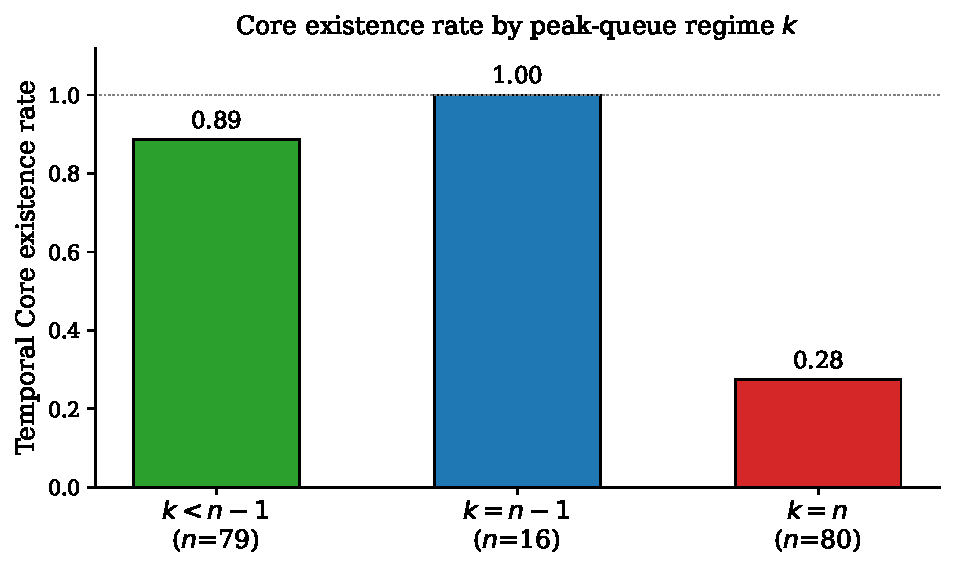
\includegraphics[width=0.7\textwidth]{fig3_core_vs_k.pdf}
\caption{Temporal Core existence rate stratified by peak-queue regime $k$. The complement-coalition mechanisms (Corollary~\ref{cor:single-complement}, Corollary~\ref{cor:balanced-complement}, Corollary~\ref{cor:balanced-near-complement}) all require $k\ge n-1$. Empirically, 58 of the 67 empty Cores concentrate at $k=n$ via single / balanced / balanced-near-complement / near-complement-residual mechanisms; the remaining 9 occur at $k<n-1$ via the intermediate-coalition mechanism of Observation~\ref{obs:intermediate}, all in patterns $\text{B}_{\text{medium}}$ or E.}
\label{fig:core-k}
\end{figure}

\paragraph{Why does the intermediate-coalition mechanism vanish under CI/BR?} A plausible explanation: under nearest-neighbor dispatch, myopic detours inflate $C(N)_{\text{online}}$ relative to $\cstar(N)$, driving the realized $r$ upward. The first-stage Core LP's dual concentrates on partition pairs $(S,N\setminus S)$ where $c(S)+c(N\setminus S)\ge r\,\cstar(N)$ becomes binding; once $r$ exceeds $r^{(P)}_S$, that pair certifies emptiness via Theorem~\ref{thm:partition-pair}. Cheapest-insertion and batch re-optimization keep $r$ closer to 1, leaving no partition pair binding in the realized $\F$. A formal queueing-theoretic characterization is left as future work (Section~\ref{sec:conclusion}, Limitation~(iv)).

\subsection{Pattern-level analysis}
\label{ssec:pattern}

Table~\ref{tab:pattern} reports the salient statistics per arrival pattern, pooled over $n$ and seeds. Figure~\ref{fig:coal-red} visualizes the relative size of $\F$.

\begin{table}[t]
\centering
\caption{Pattern-level aggregate statistics (NN policy, $5\times 5=25$ instances per pattern; overall row pools all 175 instances). $\bar r^{\ast}$, being a function of coordinates only ($r^{\ast} = \sum_i c(\{i\})/\cstar(N)$), is shared across patterns by construction (coordinates iid uniform within each cell); the pooled mean is $4.351$ and is reported as an overall value rather than per-pattern. Em-dashes in $\bar r^{\ast\ast}$ (resp.\ $\bar r^{\ast\ast\ast}$) indicate patterns where Corollary~\ref{cor:single-complement} (resp.\ Corollary~\ref{cor:balanced-complement}) is never applicable. Bracketed quantities in the Core-rate column are Wilson 95\% confidence intervals; per-pattern intervals have full width $\approx 30$--$35$ percentage points (half-width $\pm 15$--$18$ pp) reflecting the $n=25$ replicate count, and the overall interval narrows to $\approx 14$ pp full width ($\pm 7$ pp).}
\label{tab:pattern}
\small
\resizebox{\textwidth}{!}{%
\begin{tabular}{@{}lcccccccc@{}}
\toprule
Pattern & $\rho$ & Core rate [95\% CI] & $\bar r$ (sd) & $\bar r^{\ast\ast}$ (sd) & $\bar r^{\ast\ast\ast}$ & $\overline{|\F|/(2^n-1)}$ & Cor~\ref{cor:single-complement} app/fires & Cor~\ref{cor:balanced-complement} app/fires \\
\midrule
A                           & $\infty$ & 0.36 [0.20, 0.55] & 1.125 (0.102) & 1.181 (0.059) & 1.092 & 1.000 & 25 / 9  & 25 / 15 \\
$\text{B}_{\text{heavy}}$   & 4.0      & 0.20 [0.09, 0.39] & 1.233 (0.127) & 1.187 (0.061) & 1.094 & 0.985 & 25 / 15 & 24 / 20 \\
$\text{B}_{\text{medium}}$  & 2.0      & 0.56 [0.37, 0.73] & 1.273 (0.135) & 1.305 (0.148) & 1.150 & 0.590 & 13 / 3  &  7 /  4 \\
$\text{B}_{\text{light}}$   & 0.5      & 1.00 [0.87, 1.00] & 1.690 (0.210) &      ---      &  ---  & 0.077 &  0 / 0  &  0 /  0 \\
C                           & 2.0      & 0.28 [0.14, 0.48] & 1.197 (0.149) & 1.181 (0.059) & 1.087 & 0.985 & 25 / 10 & 24 / 18 \\
D                           & 1.0      & 1.00 [0.87, 1.00] & 1.332 (0.121) & 1.398 (0.217) &  ---  & 0.196 &  3 / 0  &  0 /  0 \\
E                           & 1.0      & 0.92 [0.75, 0.98] & 1.337 (0.169) & 1.505 (0.139) &  ---  & 0.273 &  5 / 0  &  0 /  0 \\
\midrule
Overall                     & ---      & 0.62 [0.54, 0.69] & 1.312 (0.224) & 1.223 (0.121) & 1.096 & 0.587 & 96 / 37 & 80 / 57 \\
\bottomrule
\end{tabular}}
\end{table}

Three regimes emerge. Patterns with $\rho\ge 2$ and saturated arrival timing (A, $\text{B}_{\text{heavy}}$, C) reach near-full feasibility ($\overline{|\F|/(2^n-1)}\ge 0.985$ for $\text{B}_{\text{heavy}}$ and C; $|\F|=2^n-1$ for A) and place Corollary~\ref{cor:single-complement} in the applicable regime for nearly every instance, firing in $9/25$, $15/25$, and $10/25$ respectively. Sparse-feasibility regimes ($\text{B}_{\text{light}}$, D, E) keep $\overline{|\F|/(2^n-1)}\le 0.27$ and render Corollary~\ref{cor:single-complement} either inapplicable or non-firing; in these regimes the mean competitive ratio rises ($\bar r\in[1.33,1.69]$) because the online tour detours to reach customers as they arrive while $\cstar(N)$ reflects the offline optimum, but Corollary~\ref{cor:cor52} blocks every complement-based mechanism and the 2 empty Cores observed in pattern E arise solely via the intermediate-coalition mechanism of Observation~\ref{obs:intermediate}.

\paragraph{Load parameter $\rho$ alone does not determine Core stability.} Patterns $\text{B}_{\text{medium}}$ and $C$ share $\rho=2$ but differ in arrival geometry; this structural difference alone yields qualitatively distinct Core stability regimes ($\text{B}_{\text{medium}}$ Core rate $0.56$ vs.\ $C$ $0.28$).


\begin{figure}[t]
\centering
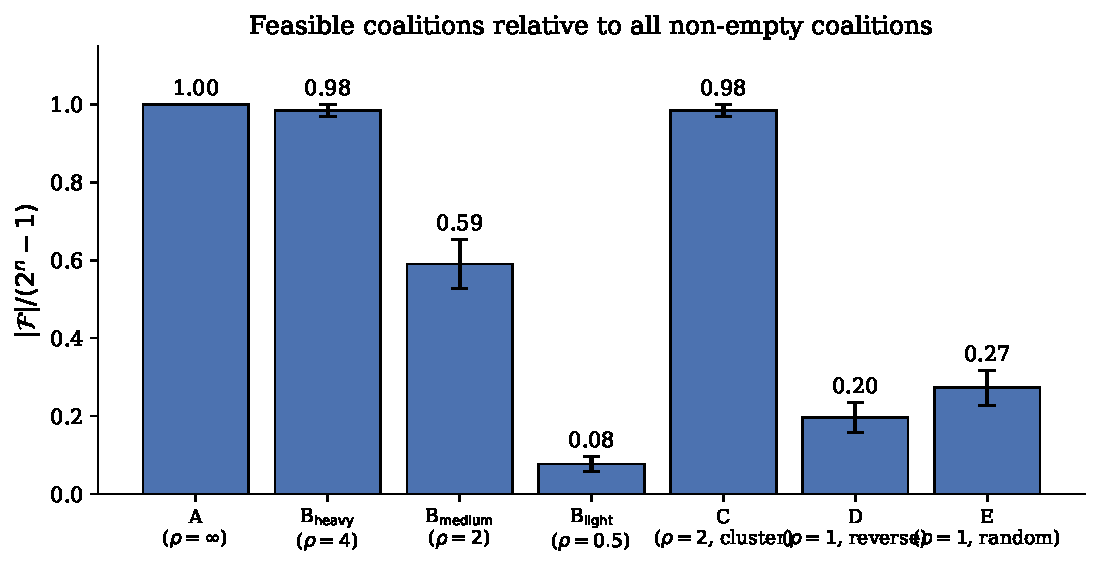
\includegraphics[width=0.85\textwidth]{fig4_coalition_reduction.pdf}
\caption{Relative size of the feasible coalition family, $|\F|/(2^n-1)$.}
\label{fig:coal-red}
\end{figure}

\subsection{\texorpdfstring{Sharpness of $r^{\ast\ast}$ versus $r^{\ast}$}{Sharpness of r** versus r*}}

Empirically, on the NN grid $\bar r^{\ast\ast}=1.223$ and $\bar r^{\ast\ast\ast}=1.096$ versus $\bar r^{\ast}=4.351$; the sharpness factors are $r^{\ast}/r^{\ast\ast} \approx 3.56$ and $r^{\ast}/r^{\ast\ast\ast} \approx 3.97$. Because the realized ratio $\bar r = 1.312$ is close to $r^{\ast\ast}$ and $r^{\ast\ast\ast}$ but far below $r^{\ast}$, Corollary~\ref{cor:single-complement} and Corollary~\ref{cor:balanced-complement} are operationally informative whereas Remark~\ref{rem:rstar} almost never fires. The classical bound grows with $n$ because $r^{\ast} = \sum_i c(\{i\})/\cstar(N)$ has a numerator scaling linearly in $n$ while $\cstar(N)$ scales like $\sqrt{n}$ on uniform planar instances; $r^{\ast\ast}$ and $r^{\ast\ast\ast}$, in contrast, are pinned near $1$ because complement coalitions $N\setminus\{i\}$ nearly partition the grand tour. This explains why the gap between the two widens with $n$ and quantifies the practical advance of the temporal analysis. Supplementary Section~\ref{app:sharpness} (Supplementary Figure~\ref{fig:rhist}) plots the three threshold distributions side by side.

\subsection{Robustness to dispatch policy}
\label{ssec:policy}

The three sufficient conditions of Section~\ref{sec:theory} have policy-independent geometric components ($c(\{i\})$, $c(N\setminus\{i\})$, $\cstar(N)$ are functions of coordinates alone); their applicability and the $\F$-dependent minima ($r^{\ast\ast}$, $r^{(P)}_{\min}$) vary with the realized $\F$. Empirically, applicability counts differ by at most one across the three dispatch policies (525 policy-instance pairs); all three thresholds preserve the no-false-positives guarantee, and the intermediate-coalition mechanism of Observation~\ref{obs:intermediate} disappears under both CI and BR. Detailed per-policy results, including the dispatch-policy contingency table and the empty-mechanism breakdown, appear in Supplementary~Section~S5.

\subsection{Scale-up to larger \texorpdfstring{$n$}{n}}
\label{ssec:scaleup}

Our main study at $n\le 15$ is capped by the $O(n^2 2^n)$ cost of Held--Karp. To test whether the theoretical and empirical findings of the preceding subsections persist at larger scales, we extend the study to $n\in\{20,30,50\}$ for three representative patterns---A ($\rho=\infty$, simultaneous), $\text{B}_{\text{medium}}$ ($\rho=2$, sequential), and C ($\rho=2$, clustered)---spanning the Core-fragile, Core-safe, and intermediate regimes. Each cell uses 5 seeds, giving 45 scale-up instances with NN dispatch.

Solver and calibration follow the methodology described in Supplementary Section~S3.

\begin{table}[t]
\centering
\caption{Scale-up aggregate statistics (5 seeds each). Em-dashes in $\bar r^{\ast\ast}$ indicate no feasible complement coalition (Corollary~\ref{cor:single-complement} vacuous). For pattern A with $n\ge 30$ the Core LP is intractable to enumerate, since $|\F|=2^n-1$; emptiness there is certified by Corollary~\ref{cor:single-complement} (conditional on LKH-computed $c^{\ast}(S)$ values for $n>20$; minimum $r-r^{\ast\ast}$ margin $0.0159$ in absolute ratio units; this is several orders of magnitude larger than the relative LKH--vs--Held--Karp calibration error of $0.000\%$ measured at $n=15$, so the analytic certification is not threatened by heuristic-solver inexactness) for the 4 of 5 seeds at $n=30$ and 5 of 5 at $n=50$ where $r>r^{\ast\ast}$, and by a restricted Core LP (Supplementary Materials Section~S3) for the one seed at $n=30$ where $r\le r^{\ast\ast}$. $\text{B}_{\text{medium}}$ rows report a one-sided sampled-LP observation only, not a proof of full Core nonemptiness (see footnote $\S$ and Finding~3(b)).}
\label{tab:scaleup}
\small
\begin{tabular}{@{}lcccccc@{}}
\toprule
Pattern & $n$ & Core rate (full/analytic) & No-viol.\ rate (sampled LP)$^{\S}$ & $\bar r$ & $\bar r^{\ast\ast}$ & $\bar k$ \\
\midrule
A                          & 20 & 0 / 5$^{\ddagger}$       & ---   & 1.167 & 1.119 & 20.0 \\
A                          & 30 & 0 / 5$^{\dagger\ddagger}$ & ---   & 1.187 & 1.096 & 30.0 \\
A                          & 50 & 0 / 5$^{\dagger}$         & ---   & 1.211 & 1.068 & 50.0 \\
\midrule
$\text{B}_{\text{medium}}$ & 20 & --- & 5 / 5$^{\S}$ & 1.330 & --- & 15.4 \\
$\text{B}_{\text{medium}}$ & 30 & --- & 5 / 5$^{\S}$ & 1.309 & --- & 23.2 \\
$\text{B}_{\text{medium}}$ & 50 & --- & 5 / 5$^{\S}$ & 1.387 & --- & 37.6 \\
\midrule
C                          & 20 & 0 / 5 & --- & 1.335 & 1.119 & 20.0 \\
C                          & 30 & 0 / 5 & --- & 1.282 & 1.096 & 30.0 \\
C                          & 50 & 0 / 5 & --- & 1.282 & 1.068 & 50.0 \\
\bottomrule
\end{tabular}

{\footnotesize $^{\dagger}$ Core LP not enumerated at this scale; Corollary~\ref{cor:single-complement} fires in $4/5$ seeds at $n=30$ and $5/5$ at $n=50$; the one non-firing seed at $n=30$ (seed 123) is certified by a restricted Core LP (Supplementary Materials Section~S3). $^{\ddagger}$ At $n=20$, Corollary~\ref{cor:single-complement} is vacuous ($r\le r^{\ast\ast}$) at seeds 99 and 123 and fires at seeds 7, 42, 256; at $n=30$, it is vacuous at seed 123 only. Core emptiness for the vacuous seeds is certified by the near-complement mechanism (Remark~\ref{rem:near-complement}, Section~\ref{ssec:cor16}). $^{\S}$ No intermediate-coalition violation detected in the sampled restricted LP of $10^{4}$ coalitions per instance; this does \emph{not} certify full Core nonemptiness (per-draw detection fraction $\approx 10^{-2}, 10^{-5}, 10^{-11}$ at $n=20$ (joint $\sim$~moderate), $n=30$ (joint $<10\%$), $n=50$ (joint $\sim 10^{-7}$, \textbf{placeholder only}) respectively). The structural statement (complement mechanisms blocked by Corollary~\ref{cor:cor52}) is analytically sharp; the no-violation observation is one-sided. The $n=50$ row should therefore be read as a placeholder for ``intractable to test in the current methodology'' rather than as a positive nonemptiness claim; only the structural blocking via Corollary~\ref{cor:cor52} carries asymptotic strength at $n=50$. The $n=20$ companion is informative (joint detection probability above $50\%$ under reasonable concentration of the binding partition pair), the $n=30$ companion is weakly indicative (joint detection still under $10\%$), and the $n=50$ companion is uninformative. At $n>15$ the Core-existence judgment is made via the restricted LP of Supplementary Materials Section~S3 rather than full $2^n-1$ enumeration.}
\end{table}

Four findings emerge.

\paragraph{Finding 1: $\bar r^{\ast\ast}$ decays with $n$, confirming Theorem~\ref{thm:asymptotic}.} For Pattern~A, $\bar r^{\ast\ast}$ drops from $1.181$ at $n=15$ to $1.119, 1.096, 1.068$ at $n=20, 30, 50$ (Pattern~C exhibits the same decay; $\text{B}_{\text{medium}}$ has no feasible complement at any scale). A log-log regression of $\bar r^{\ast\ast}-1$ on $n$ for Pattern~A yields slope $-0.54$ ($R^2=0.99$, all 8 per-$n$ mean points) and $-0.62$ ($R^2=1.00$, scale-up subset $n\in\{15,20,30,50\}$), close to Theorem~\ref{thm:asymptotic}'s $-1/2$ and partway toward Remark~\ref{rem:asymptotic-tighter}'s $-1$.

\paragraph{Finding 2: Pattern C activates the complement mechanism as $n$ grows.} On the main grid ($n\le 15$), Pattern~C's $\bar r = 1.197$ is only marginally above $\bar r^{\ast\ast}=1.181$ (Core-existence $28\%$). By $n=20$ the gap widens to $\bar r=1.335$ vs.\ $\bar r^{\ast\ast}=1.119$, and all 5 instances are empty (same at $n=30,50$). Two concurrent effects drive this: $\bar r$ rises as the NN competitive ratio degrades and the clustered zig-zag accumulates waiting, while $\bar r^{\ast\ast}$ falls by Theorem~\ref{thm:asymptotic}.

\paragraph{Finding 3: Pattern $\text{B}_{\text{medium}}$ blocks the complement mechanism structurally at every scale; intermediate-coalition violations are not detected in the sampled LP but cannot be ruled out.} We split this finding into an analytically sharp structural claim (a) and a one-sided empirical observation (b) whose detection power decreases with $n$.

\emph{(a) Structural claim (analytic, strong).} Across $n\in\{20,30,50\}$, $\text{B}_{\text{medium}}$'s sparse arrivals keep $\bar k$ strictly below $n-1$ ($\bar k = 15.4, 23.2, 37.6$), so every complement $N\setminus\{i\}$ is infeasible and all three complement-based mechanisms (Corollary~\ref{cor:single-complement}, Corollary~\ref{cor:balanced-complement}, and Corollary~\ref{cor:balanced-near-complement}) are structurally blocked by Corollary~\ref{cor:cor52}, regardless of the realized $r$.

\emph{(b) Empirical observation (one-sided, weak; see detection-limit warning below).} Across the 15 instances at $n\in\{20,30,50\}$, $\bar r \in [1.31,1.39]$; no intermediate-coalition violation is observed in our sampled restricted-LP of $K=10^{4}$ coalitions per instance. This is a one-sided certificate only: the sampled LP cannot conclude full Core nonemptiness, and the sampling fraction $K/(2^{n}-1)$ collapses as $n$ grows ($\approx 10^{-2}, 10^{-5}, 10^{-11}$ at $n=20,30,50$). Absence of observed violation at $n=50$ is therefore not evidence of rarity.

\paragraph{Detection-limit warning ($n=50$).} The per-draw detection probability is $\sim 10^{-11}$ at $n=50$, $\sim 10^{-5}$ at $n=30$, and $\sim 10^{-2}$ at $n=20$, so Finding~3(b) is uninformative at $n=50$ (a placeholder for ``intractable to test''), weakly indicative at $n=30$, and informative at $n=20$. Only the structural claim 3(a) carries asymptotic strength.

\paragraph{Finding 4: Near-complement-to-Theorem-9 transition at seed 123.} Seed 123 under Pattern~A exhibits a transition consistent with Theorem~\ref{thm:asymptotic}'s $O(n^{-1/2})$ tightening of $r^{\ast\ast}$: at $n=20,30$, $r<r^{\ast\ast}$ and Core emptiness is certified by the near-complement mechanism (Remark~\ref{rem:near-complement}) via a restricted Core LP; at $n=50$, $r^{\ast\ast}$ has tightened sufficiently that Corollary~\ref{cor:single-complement} fires directly. Detailed per-seed binding-size distributions and the restricted-LP methodology are in Supplementary Materials Section~S3.

\paragraph{Intractability of Pattern A at $n\ge 30$.} For Pattern~A, $|\F|=2^n-1$ ($\sim 10^9$ at $n=30$, $\sim 10^{15}$ at $n=50$), beyond enumeration. Corollary~\ref{cor:single-complement} nevertheless certifies emptiness in 12 of 15 seed--size combinations a priori (Table~\ref{tab:scaleup}); the three exceptions (seeds 99, 123 at $n=20$; seed 123 at $n=30$) are certified by the restricted Core LP of Supplementary Materials Section~S3 (Finding~4 above). The intractability regime is thus precisely where Corollary~\ref{cor:single-complement} (with Remark~\ref{rem:near-complement} backup) suffices without enumeration.

\paragraph{Summary.} The qualitative findings persist to $n=50$: pattern C's Core-empty tail becomes near-certain by $n=20$ via Theorem~\ref{thm:asymptotic}'s $r^{\ast\ast}$ tightening, while Corollary~\ref{cor:cor52}'s structural safeguard only strengthens ($\bar k<n-1$ blocks complement mechanisms at every scale-up cell). For $\text{B}_{\text{medium}}$ at $n=50$, only the structural claim of Finding~3(a) survives as an asymptotic conclusion; the sampled-LP companion of Finding~3(b) is detection-power limited and consistent with the main-grid observation that intermediate empties vanish under CI/BR (Section~\ref{ssec:policy}).

\section{Conclusions and future research}
\label{sec:conclusion}

We introduced the Online Traveling Salesman Game and defined the Temporal Nucleolus as the lexicographic excess minimizer over the restricted family $\F$ of coalitions realizable under the online arrival process. The classical (static) TSG is recovered at the boundary case of simultaneous arrivals; the Temporal Core is empty whenever the competitive ratio exceeds any of three complement-based thresholds (Corollary~\ref{cor:single-complement}, Corollary~\ref{cor:balanced-complement}, Corollary~\ref{cor:balanced-near-complement}) or the unifying partition-pair certificate of Theorem~\ref{thm:partition-pair}; a bounded waiting queue ($k<n-1$) structurally blocks the three complement-based mechanisms (Corollary~\ref{cor:cor52}), but not the partition-pair mechanism via non-singleton splits. On the 175-instance NN grid, the four analytic thresholds jointly certify 66 of 67 observed empty Cores with no false positives---1 near-complement residual completes the five-mechanism decomposition. The thresholds are sharper than the classical bound by $3.56\times$ ($\bar r^{\ast\ast}=1.223$) and $3.97\times$ ($\bar r^{\ast\ast\ast}=1.096$), making them the first operationally informative thresholds for cost-sharing stability in online routing.

\paragraph{Platform-design implication.} From a platform-design perspective, our results offer suggestive evidence that enforcing short service-time promises---equivalently, keeping the peak queue depth below $n-1$---structurally rules out all three complement-coalition mechanisms for emptying the Core. In the shallow-queue regime, the partition-pair mechanism of Theorem~\ref{thm:partition-pair} remains logically possible (Observation~\ref{obs:intermediate}), and is empirically observed only under nearest-neighbor dispatch: cheapest-insertion and batch re-optimization produce zero such cases in our grid, suggesting that even moderately informed dispatch policies mitigate this mechanism (Section~\ref{ssec:policy}).

\paragraph{Operational trade-offs.} Bounding $k<n-1$ in practice requires tighter service-time commitments, larger fleet capacity, or more frequent dispatch---each with resource costs not quantified by the cooperative-game analysis here. Moreover, $k$ is endogenous to arrival and service rates rather than a free control variable, so high-volume platforms may face $k=n$ regimes even under aggressive dispatching. Combining the cooperative game with explicit fleet-capacity costs along the lines of \citet{ozener2008allocating} would clarify this trade-off.

\paragraph{Limitations and future work.} Five concerns merit explicit comment.
\begin{enumerate}[label=(\roman*),leftmargin=*,itemsep=2pt,topsep=2pt]
\item \emph{Dispatch policy.} Theorems and corollaries depend on the
  realized $(r,\F,k)$: the geometric coalition costs are
  policy-independent, but $\F$ itself, applicability, and
  $\F$-restricted minima depend on the dispatch policy through
  realized service times. Empirical robustness across NN/CI/BR is
  shown; learning-based or forecasting-aware policies remain open.
\item \emph{Instance scale.} Section~\ref{ssec:scaleup} extends to
  $n\in\{20,30,50\}$ via LKH (calibration error $0.000\%$ vs.\
  Held--Karp at $n=15$, well below the minimum $r-r^{\ast\ast}$ margin
  of $0.0159$). For $\text{B}_{\text{medium}}$ at $n=50$, the
  sampled-LP companion is uninformative (Finding~3(b)); only the
  structural blocking via Corollary~\ref{cor:cor52} carries asymptotic
  strength. Extending to $n\ge 100$, non-uniform geometries,
  heavy-tailed queueing, and full-$\F$ certification is open.
\item \emph{Near-complement residual.}
  Corollary~\ref{cor:balanced-near-complement} closes 9 of 10
  main-grid near-complement cases; the residual ($n=15$, A, seed 42)
  misses the strict inequality by $\approx 2\times 10^{-3}$. Whether
  enlarging the balancing family or relaxing to a covering inequality
  closes this gap is open.
\item \emph{Intermediate-coalition mechanism.}
  Theorem~\ref{thm:partition-pair} certifies the 9 cases of
  Observation~\ref{obs:intermediate} via dual-support extraction; a
  policy-aware predictive condition derived from queueing primitives
  (peak queue $k$, occupancy autocorrelation, dispatch greediness)
  that predicts which arrival--service realizations admit a binding
  partition pair, rather than after-the-fact LP dual extraction,
  remains open. The mechanism is also policy-sensitive: observed only
  under NN, absent under CI/BR.
\item \emph{Policy-dependence of $\F$.} The per-coalition cost values
  $c(S)$ are policy-independent (geometric); the family $\F$ depends
  on realized service times and hence on the dispatch policy, and
  thus the applicability and the $\F$-restricted minima
  ($r^{\ast\ast}$, $r^{(P)}_{\min}$) are policy-dependent. A
  counterfactual framing in which $\F$ depends only on arrival times
  is left for future work.
\end{enumerate}

\emph{Scope demarcation and Online VRG.} The single-vehicle scope isolates the temporal coalition-feasibility structure of $\F$ from fleet-assignment confounds (the insertion identity $c(\{i\})+c(N\setminus\{i\})\ge\cstar(N)$ underlying our complement-based sufficient conditions can fail under capacity-binding multi-vehicle costs; see §1 ``Why single vehicle''). An \emph{Online Vehicle Routing Game} combining $\F$ with multi-vehicle capacity \citep{gothe1996vrg,engevall2004heterogeneous}, capacitated coalition costs, and rolling-horizon consistency \citep{lehrer2013dynamic,kimms2016rolling} is identified as future work.

\section*{Acknowledgements}
This work was supported by the Korea Institute of Industrial Technology under Grant No.~EH-26-0002.

\paragraph*{Declaration of generative AI in scientific writing.} During the preparation of this work the authors used Claude (Anthropic) for language editing and analysis-script drafting; the authors reviewed and edited the content and take full responsibility for it.

\section*{Data and code availability}
All code, data, and reproducibility scripts are publicly available at \url{https://github.com/sage-Tae/online-tsg-2026}.

%% Bibliography (EJOR style; references_ejor.bib has Arroyo Crossref note stripped)
%% References-only typography compression for the 30-page EJOR cap.
%% Single-spacing applied to bibliography only; main body remains
%% one-and-a-half-spaced. Inter-entry skip tightened from default.
\renewcommand{\bibfont}{\footnotesize}
\setlength{\bibsep}{0pt plus 0.0ex minus 0.0ex}
\begin{spacing}{0.85}
\bibliographystyle{apalike-ejor}
\bibliography{references_ejor}
\end{spacing}

\end{document}
